\documentclass[9pt]{extarticle}
\usepackage[utf8]{inputenc}
\usepackage[T1]{fontenc}
\usepackage[hidelinks]{hyperref}
\usepackage{amsmath,amssymb,amsthm}
\usepackage{graphicx}
\graphicspath{{figures/}}
\usepackage[numbers]{natbib}

\title{Safe Active Discrimination of Fractional, Delayed, and Finite Latent Memory in a Strong-Allee Predator--Prey Model}
\author{Ibrahim Alraddadi\\
Department of Mathematics, Faculty of Science\\
Islamic University of Madinah, Madinah, Saudi Arabia\\
\texttt{ialraddadi@iu.edu.sa}}
\date{\today}

\begin{document}
\maketitle

\begin{abstract}
We study how controlled ecological experiments can distinguish Caputo memory from integer-order, delayed, and finite latent alternatives in a strong-Allee predator--prey system. The ecological backbone is intentionally inherited from our previously submitted companion paper: the same strong-Allee model, locked parameters, coexistence equilibrium, and Jacobian are reused as the experimental test bed and are explicitly not claimed as new contributions here. The main text is organized around four analytical results and an expanded numerical study. Structurally, the collocated Caputo transfer has a noninteger high-frequency signature that cannot be exactly reproduced by the declared finite latent or retarded-delay classes. Practically, finite exponential mixtures approximate fractional memory over finite horizons, producing a complexity-dependent testing obstruction. Directly on the ecological prey channel, interval arithmetic certifies finite-state approximations whose error decreases from $0.5335$ at $m=4$ to $0.0070$ at $m=32$ for $\alpha=0.85$, $A=0.25$, and $T=12$; under the declared pulse budget, the associated Gaussian testing lower bound approaches chance. We then introduce a combined fractional-delay model that reduces to the pure Caputo case at $\tau=0$ and to the DDE case at $\alpha=1$. New simulations show that delay systematically shifts the predator peak, erodes the Allee safety margin, and creates intermediate responses that are not well represented by either pure limit. Across six perturbation families and a large four-class benchmark, broadband inputs improve discrimination but cross the Allee threshold more frequently, whereas transient inputs are safer numerically but less informative. The results expose a fundamental safety--informativeness trade-off in experimental identification of ecological memory.
\end{abstract}

\theoremstyle{plain}
\newtheorem{theorem}{Theorem}[section]
\newtheorem{lemma}[theorem]{Lemma}
\newtheorem{corollary}[theorem]{Corollary}
\theoremstyle{definition}
\newtheorem{definition}[theorem]{Definition}
\theoremstyle{remark}
\newtheorem{remark}[theorem]{Remark}

\section{Introduction}
\label{sec:introduction}

Caputo derivatives of order $0<\alpha<1$ model hereditary effects in viscoelasticity, anomalous transport, and population dynamics~\cite{F01,F02,F03,F04}; fractional predator--prey models in particular form a sizeable literature~\cite{E06,E07,E08,E09}. An empirical difficulty sits underneath all of it. Estimating $\alpha<1$ from data does not establish a fractional mechanism, because on a bounded window $[0,T]$ a delay term $\xi(t-\tau)$ or a low-dimensional latent state $q\in\mathbb{R}^m$ generates trajectories within the noise floor of the fractional ones (Corollary~\ref{cor:closure} makes this quantitative). Design methods for fractional-order \emph{estimation} exist~\cite{FOED01,FOED02,FOED03,FOED04}; safety-constrained information acquisition has been analyzed in general settings~\cite{SAFE26A,SAFE26B}. The intersection --- discrimination between memory \emph{mechanisms}, under an ecological safety constraint --- is the subject here:

\begin{quote}
\emph{Which perturbations and measurements can distinguish fractional memory from delayed or latent alternatives in a strong-Allee ecological system, and when does ecological safety make that discrimination fundamentally difficult?}
\end{quote}

Safety is not decorative in this question. Below the Allee threshold $A$ the prey growth term $P(x)=rx(1-x/K)(x/A-1)$ turns negative and collapse is irreversible, so the perturbations most informative about memory ($\|u\|_\infty$ near the budget, broadband spectra) are the ones most likely to destroy the object of study. Section~\ref{sec:benchmark} measures this numerically: among the six classical excitation families, the best-discriminating input crosses the threshold in $100\%$ of stable-regime cells. Section~\ref{subsec:safe-search} then shows that this apparent conflict is a property of those families rather than of the ecology.



\paragraph{Provenance of the ecological backbone.}
The ecological backbone follows the companion certification study~\cite{P01}: the equations, locked parameters, coexistence equilibrium and Jacobian are restated here for self-containment and are not claimed as contributions of the present work. That study certifies dynamical regimes of a specified Caputo model; it does not address whether such a model can be told apart from a delayed or latent mechanism reproducing the same observations to within $\sigma$, which is the question posed here. No result below recertifies the backbone. With the ecology frozen, differences between simulated observations are attributable to the memory law or to the experiment, never to an altered population model. Only the integer-order and Caputo mechanisms share $J(A)$ exactly; the delayed and latent rivals are calibrated alternative response laws matched at the same operating point, input channel and units.

\paragraph{Main contributions.}
The paper is organised around one falsification and one positive design result, with a separate obstruction that survives both.

\begin{enumerate}
    \item \textbf{Safe waveforms outside the classical families outperform every classical baseline} (Section~\ref{subsec:safe-search}). Under the same peak-amplitude budget $\|u\|_\infty\le0.100$ and a hard Allee-margin constraint, a constrained search over $163\,840$ candidate waveforms returns piecewise-constant designs with four-class BIC macro-accuracy $0.803$ and zero observed threshold crossings, against $0.514$ for the only classical family that is safe at this budget and $0.763$ for the best classical design of any kind, which crosses in $35.7\%$ of cells. The gain is concentrated where the safe classical design fails: Caputo recall rises from $0.404$ to $0.911$, delay recall from $0.445$ to $0.853$.
    \item \textbf{The six-family safety--informativeness frontier is not a property of the system} (Sections~\ref{subsec:amplitude}--\ref{subsec:safe-search}). Reducing amplitude does not restore safety --- the leading design still crosses in $71.4\%$ of cells at half amplitude, while its realised response gain rises to $4.86$ times the linear certificate, the signature of basin escape rather than linear response. The severe frontier reported for classical excitation families is therefore a statement about that parameterisation. A Pareto cost remains: the best unsafe candidate separates the hypotheses substantially better than the best safe one, so safety is not free.
    \item \textbf{A separate finite-horizon latent-complexity obstruction, quantified at response level to $m=128$} (Sections~\ref{subsec:semantics}--\ref{subsec:state}). Computed directly on the prey response rather than inferred from the memory kernel, the $L^1$ surrogate error falls to $4.8\cdot10^{-5}$ at $m=128$ and the induced exact minimax testing floor reaches $0.49999$: at attainable latent orders the finite-state rival is indistinguishable under the declared protocol, for every input in the budget. Waveform search does not remove this. In the benchmark the leading safe design also recovers only $0.475$ recall against the finite-latent rival, which is consistent with the obstruction but not evidence for it: the BIC penalty on the higher-dimensional model is an alternative explanation that this study does not separate.
    \item \textbf{Trajectory safety status, stated exactly} (Sections~\ref{sec:design} and~\ref{sec:benchmark}). Safety of the reported designs is verified a posteriori by mesh refinement together with a rigorous inter-node modulus; for four of the eight headline trajectories a validated enclosure with self-consistent error control is obtained, and only those are called rigorous. Constants entering the nonlinear invariant-set route are interval-certified, and that route is shown to admit inputs $70$ times smaller than the amplitude actually used.
    \item \textbf{Reproducibility control.} The frozen four-class benchmark reproduces to four decimal places on an independent host under a re-implemented driver ($2268$ cells across three amplitudes, no solver divergences).
\end{enumerate}

Contributions 1, 2 and 5 are empirical, established by the benchmark and the search; contribution 3 combines a proved bound (Theorem~\ref{thm:T20}) with computed surrogate errors, interval-enclosed for $m\le32$ and high-accuracy numerical for $m=64,128$; contribution 4 is a verification result whose exact status is stated per trajectory in Section~\ref{sec:benchmark}.

The structural separation of Section~\ref{sec:analysis} and the positive exponential-sum approximation it is contrasted with are \emph{not} contributions: the former is classical fractional-systems material, and the latter is the construction of McLean~\cite{K07} building on Beylkin and Monz\'on~\cite{K03,K04}. We record only an endpoint-inclusive $L^1(0,T)$ variant with the exact horizon scaling the convolution argument requires (Lemma~\ref{lem:soe}), and attribute the technique where it is used.

Complete proofs, secondary results, the Bayesian sequential extension, and solver derivations are in the Supplementary Material; the main text keeps the four statements needed to read the numerics.

\begin{figure}[htbp]
\centering
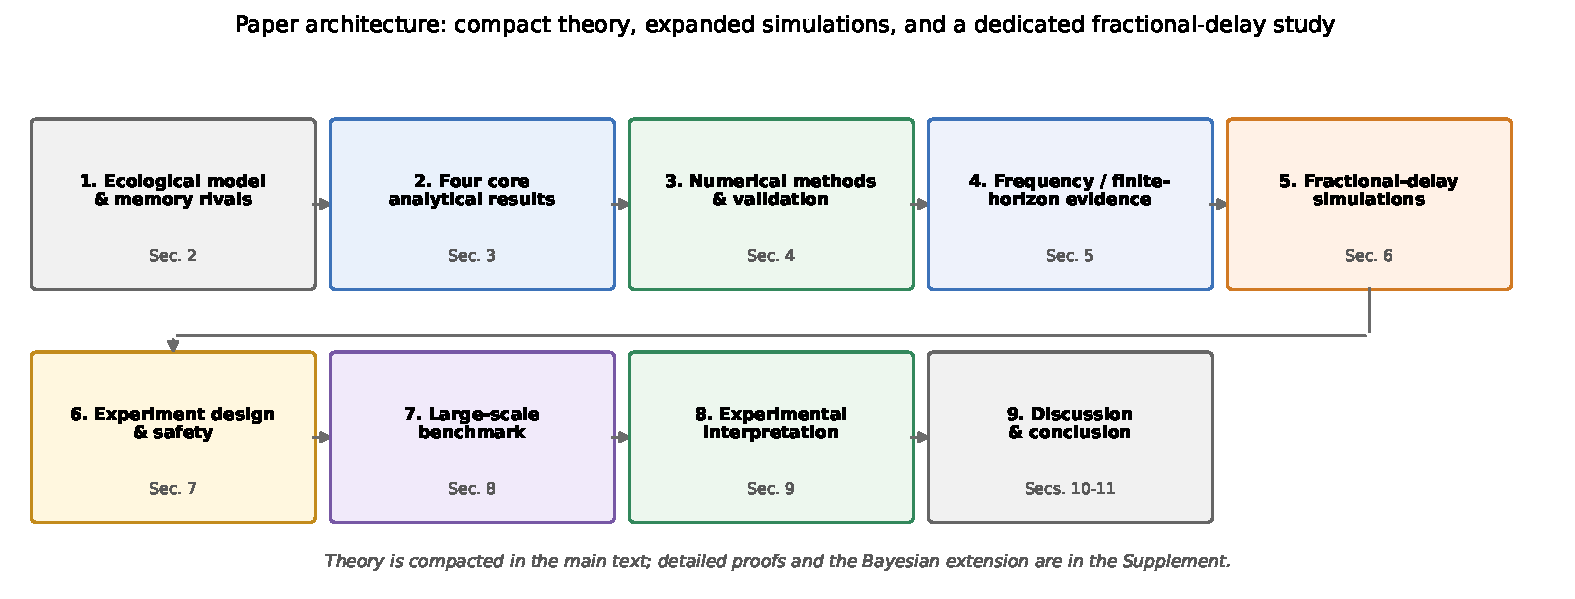
\includegraphics[width=0.98\textwidth]{fig17_paper_workflow}
\caption{Structure of the paper. Sections~\ref{sec:model}--\ref{sec:analysis}: ecological model, rival memory laws, and the four analytical results. Sections~\ref{sec:numerics}--\ref{sec:response}: solver validation (Table~\ref{tab:solver-validation}) and frequency/finite-horizon evidence. Section~\ref{sec:fd}: fractional-delay simulations. Sections~\ref{sec:design}--\ref{sec:benchmark}: input design, safety, and the 1512-cell benchmark. Proofs and secondary theory: Supplementary Material.}
\label{fig:workflow}
\end{figure}

\section{Ecological Model and Competing Memory Mechanisms}
\label{sec:model}

\subsection{Strong-Allee predator--prey backbone}
All objects in this subsection are inherited from~\cite{P01}, where they were derived and certified with validated numerics: the model, the locked parameters, the equilibrium $(x^*,y^*(A))$, the Jacobian $J(A)$, and the Matignon boundary $\alpha^*(A)$. They are restated because the experiments of Sections~\ref{sec:numerics}--\ref{sec:benchmark} are defined in terms of them; none is claimed as new.

The nonlinear model is
\begin{align}
 f_1(x,y) &= r x\left(1-\frac{x}{K}\right)\left(\frac{x}{A}-1\right)-\frac{axy}{1+hx},\\
 f_2(x,y) &= e\frac{axy}{1+hx}-my,
\end{align}
with locked parameters
\[
r=\frac32,\qquad K=1,\qquad a=1,\qquad h=\frac12,\qquad e=\frac45,\qquad m=\frac25.
\]
The coexistence equilibrium and Jacobian are
\[
x^*=\frac23,\qquad y^*(A)=\frac{2(2-3A)}{9A},
\]
\[
J(A)=\begin{pmatrix}
\dfrac{7A-2}{8A} & -\dfrac12\\[1ex]
\dfrac{2-3A}{10A} & 0
\end{pmatrix}.
\]
For the commensurate Caputo model, local stability follows Matignon's sector condition $|\arg\mu|>\alpha\pi/2$ on the eigenvalues $\mu$ of $J(A)$~\cite{F05}. In the complex-pair regime $2/7<A<10/19$ the critical order is
\[
\alpha^*(A)=\frac{2}{\pi}\arctan\!\left(\frac{\sqrt{4D(A)-T(A)^2}}{T(A)}\right),
\]
where $T(A)=\operatorname{tr}J$ and $D(A)=\det J$. At $A=0.30$, $\alpha^*\approx0.969012276$: the Caputo system with $\alpha=0.9<\alpha^*$ is stable while its integer-order limit ($\alpha=1>\alpha^*$) is unstable~\cite{P01}. Most discrimination experiments below use $A\le2/7$, where every candidate mechanism is stable at the operating point and stability cannot serve as a discrimination shortcut.

\paragraph{Inherited backbone versus new experimental layer.}
Notation is kept identical to~\cite{P01} for an identification reason: if the ecological equations changed between papers, a difference in simulated observations could reflect the altered biology instead of the memory law. The ecology is therefore frozen and only the response law varies --- ${}^CD_t^\alpha$, the delay $\xi(t-\tau)$, or a latent state $q\in\mathbb{R}^m$ --- with all candidates facing the same budget $\|u\|_\infty\le0.10$, horizon $T=12$, and threshold $A$. Table~\ref{tab:locked-backbone} lists the frozen quantities.

\begin{table}[htbp]
\centering
\caption{Locked ecological backbone used by both manuscripts. These values are inherited inputs, not new contributions of the present paper.}
\label{tab:locked-backbone}
\small
\begin{tabular}{lll}
\hline
\textbf{Quantity} & \textbf{Value} & \textbf{Role in present experiments}\\
\hline
$r$ & $1.5$ & intrinsic prey growth\\
$K$ & $1$ & prey carrying capacity\\
$a$ & $1$ & attack-rate scale\\
$h$ & $0.5$ & Holling-II handling parameter\\
$e$ & $0.8$ & conversion efficiency\\
$m$ & $0.4$ & predator mortality\\
$x^*$ & $2/3$ & common coexistence prey level\\
$y^*(A)$ & $2(2-3A)/(9A)$ & coexistence predator level\\
$J(A)$ & Eq. above & ODE/Caputo local ecological generator\\
\hline
\end{tabular}
\end{table}

The threshold $A$ has two roles. First, $x(t)<A$ defines the failure event: $P(x)<0$ there, and the trajectory can leave the coexistence basin permanently (Figure~\ref{fig:backbone}, left). Second, $x^*-A$ is the natural safety margin; at $A=0.25$ it equals $2/3-0.25\approx0.417$. An input can thus score highly on the information criterion of Section~\ref{sec:design} and still be ecologically inadmissible --- Tables~\ref{tab:benchmark-safety} and~\ref{tab:fd-design-ranking} quantify exactly this.

\begin{figure}[htbp]\centering
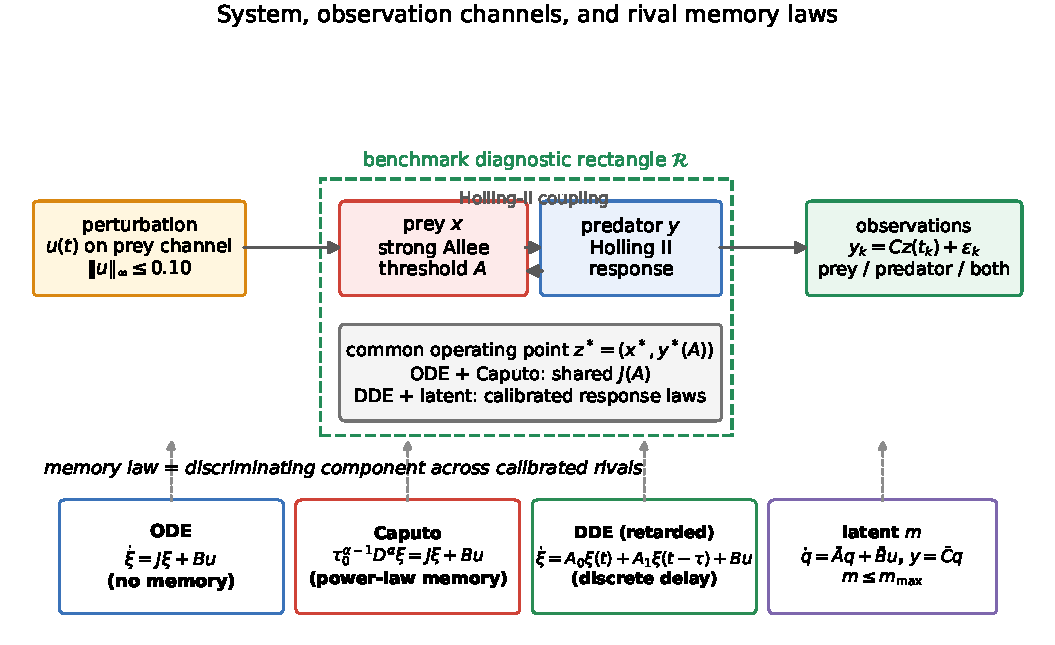
\includegraphics[width=0.98\textwidth]{fig11_system_schematic}
\caption{Setting: backbone from~\cite{P01}; perturbation $u(t)$ on the prey channel with $\|u\|_\infty\le0.10$; observations $y_k=Cz(t_k)+\varepsilon_k$ on prey, predator, or both. ODE and Caputo share $J(A)$ exactly; DDE and latent are calibrated rival response laws. Dashed rectangle: numerical benchmark diagnostic region only (not an invariant-set certificate).}
\label{fig:schematic}
\end{figure}

\begin{figure}[htbp]\centering
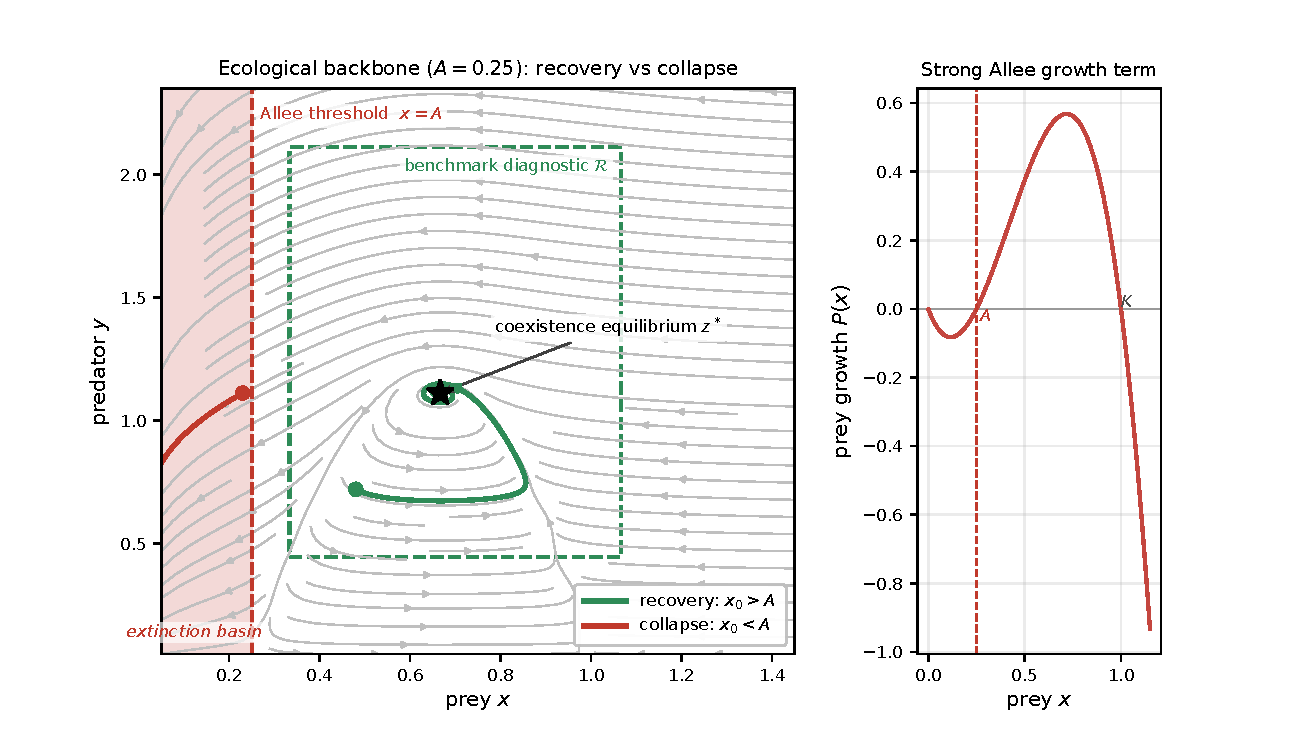
\includegraphics[width=0.94\textwidth]{fig12_backbone_regime}
\caption{Safety geometry at $A=0.25$ (backbone from~\cite{P01}). Left: recovery for $x_0>A$ versus collapse for $x_0<A$. Right: $P(x)=rx(1-x/K)(x/A-1)$, with sign change at $x=A$.}
\label{fig:backbone}
\end{figure}

\subsection{Four rival mechanisms}
With the reference time $\tau_0$ enforcing dimensional consistency~\cite{F02,F03,F04}, the four candidate mechanisms around the operating point are
\begin{align*}
\text{ODE:}&\quad \dot\xi=J\xi+Bu,\\
\text{Caputo:}&\quad \tau_0^{\alpha-1}{}^CD_t^\alpha\xi=J\xi+Bu,\\
\text{DDE:}&\quad \dot\xi=A_0\xi(t)+A_1\xi(t-\tau)+Bu,\\
\text{latent:}&\quad \dot q=\bar A q+\bar Bu,\qquad y=\bar Cq.
\end{align*}
The Caputo mechanism is the only one carrying a fractional order. The latent class, which would otherwise be flexible enough to imitate anything, is held to an explicit state-dimension budget $m$ --- a restriction whose necessity is precisely the content of Result~II below. In the benchmark the latent \emph{hypothesis} is fixed at $m=3$ while latent \emph{data} are generated at $m=1$ and $m=3$; class-wise statistics for that class are therefore pooled over the two generators, and are labelled \emph{finite-latent} rather than \emph{latent-3} wherever this matters.

\paragraph{Combined fractional-delay stress-test model.}
A system may carry hereditary memory and a trophic lag simultaneously, so we also simulate the combined model
\begin{align}
\tau_0^{\alpha-1}{}^CD_t^\alpha x(t)
&=P(x(t);A)-\frac{a x(t)y(t)}{1+h x(t)}+u(t),\\
\tau_0^{\alpha-1}{}^CD_t^\alpha y(t)
&=e\frac{a x(t-\tau)y(t)}{1+h x(t-\tau)}-m y(t),
\label{eq:fdmodel}
\end{align}
with constant equilibrium history on $[-\tau,0]$. Its boundaries are exact: at $\tau=0$, \eqref{eq:fdmodel} is the pure Caputo model; at $\alpha=1$ it is the retarded DDE benchmark. Both limits are verified numerically to $6.75\times10^{-6}$ and better in Table~\ref{tab:solver-validation}. The model is a numerical stress test only; no theorem depends on it.

\section{Analytical Backbone: What Is Proved, What Is Borrowed, What Is Computed}
\label{sec:analysis}

This section fixes the mathematics the experiments rest on. Each item is labelled by status: \emph{foundation} (standard, restated for self-containment, no priority claimed), \emph{borrowed tool} (prior art, attributed), \emph{proved here}, or \emph{computed} --- and, for computed quantities, whether the number is an interval enclosure or a high-accuracy floating-point evaluation. Three error objects recur and are never interchanged: the memory-kernel error, the induced response-operator error, and the fixed-input discrepancy (Section~\ref{subsec:semantics}).

\subsection{Result I: exact structural separation (foundation)}
The collocated Caputo transfer of the linearisation at $(x^*,y^*(A))$ carries an $O(\omega^{-\alpha})$ high-frequency signature. No finite rational latent transfer (integer-order rolloff) and no strictly proper retarded-delay model ($O(\omega^{-1})$) reproduces it exactly on an open frequency set. The mechanism --- a branch point of $s^\alpha$ at the origin against the meromorphy of the rival classes --- is classical fractional-systems material~\cite{F02,F03,F08}; no novelty is claimed for it. It is stated because it delimits what the later results can and cannot mean.

\begin{theorem}[Structural separation]
\label{thm:T4}
Let $CB\neq0$ and $\alpha\in(0,1)$ with $\alpha\notin\mathbb{Q}$ in the sense that no effectively present exponent of $s^\alpha$ is an integer multiple of $1/\alpha$. Then $G_\alpha$ is not meromorphic in any neighbourhood of $s=0$, hence differs from every finite rational transfer and from every strictly proper retarded-delay transfer.
\end{theorem}

The statement concerns exact equality of transfers on open frequency sets. It promises nothing about experiments with finite bandwidth, finite horizon $T<\infty$ and noise $\sigma>0$. That regime is governed by Lemma~\ref{lem:soe} and its corollary.

\subsection{Result II: positive exponential-sum approximation (borrowed tool)}
\label{subsec:soe}
The Caputo kernel $k_\alpha(t)=t^{\alpha-1}/\Gamma(\alpha)$ has the Stieltjes representation $k_\alpha(t)=c_\alpha\int_0^\infty\lambda^{-\alpha}e^{-\lambda t}\,d\lambda$ with $c_\alpha=\sin(\pi\alpha)/\pi$. Discretising it by the trapezoidal rule on a logarithmic grid $\lambda_k=e^{kh}$ and truncating produces an exponential sum with \emph{positive} weights and rates.

\begin{quote}
\textbf{Attribution.} This construction is prior art. Positive exponential-sum approximation of $t^{-\beta}$ by quadrature of an integral representation, including the positivity of the weights and the root-exponential order in the number of terms, is due to McLean~\cite{K07}, building on the exponential-sum approximation theory of Beylkin and Monz\'on~\cite{K03,K04}; the same construction underlies the fast Caputo evaluation of Jiang et al.~\cite{K05}. The quadrature estimate we invoke is the analytic-strip trapezoidal bound~\cite{K08}, and root-exponential order is the expected optimal order for an algebraic branch point~\cite{K09}. We claim no new approximation method, no new rate law, and no priority for positive weights.
\end{quote}

What we add is narrow and technical: the published estimates are stated on a compact interval $[\delta,T]$ with $\delta>0$, excluding the singularity at the origin, whereas the discrimination argument of Section~\ref{subsec:testing} needs the convolution norm $L^1(0,T)$ \emph{including} $t=0$. The strip bound is $t$-integrable there because $\alpha>0$, so no excision is required.

\begin{lemma}[Endpoint-inclusive $L^1$ estimate and exact horizon scaling]
\label{lem:soe}
Let $E_m^+(\alpha,T)$ denote the least $L^1(0,T)$ error of an $m$-term exponential sum with positive weights and rates. Then
\begin{equation}
E_m^+(\alpha,T)=T^\alpha E_m^+(\alpha,1),
\label{eq:scaling}
\end{equation}
and for every $c<\pi\sqrt{\alpha(1-\alpha)}$ there exists $A(\alpha,c)<\infty$ with
\begin{equation}
E_m^+(\alpha,T)\le A(\alpha,c)\,T^\alpha e^{-c\sqrt m}\qquad(m\ge1).
\label{eq:rootexp}
\end{equation}
Consequently $m(\varepsilon)=O(\log^2(1/\varepsilon))$ terms suffice for accuracy $\varepsilon$.
\end{lemma}

\begin{proof}
Equation~\eqref{eq:scaling} is exact: substituting $t=Ts$ and using $k_\alpha(Ts)=T^{\alpha-1}k_\alpha(s)$ turns the $L^1(0,T)$ error into $T^\alpha$ times the $L^1(0,1)$ error, and $(c_j,\lambda_j)\mapsto(T^{1-\alpha}c_j,T\lambda_j)$ is a bijection of the admissible positive mixtures. For~\eqref{eq:rootexp} put $\lambda=e^x$, so $k_\alpha(t)=c_\alpha\int_{\mathbb R}g(x,t)\,dx$ with $g(x,t)=e^{(1-\alpha)x}e^{-te^x}$. For $|\operatorname{Im}x|\le d<\pi/2$ one has $|g|\le e^{(1-\alpha)x}e^{-te^x\cos d}$, whence the strip norm obeys $N(g(\cdot,t),d)\le2(\cos d)^{\alpha-1}\Gamma(1-\alpha)t^{\alpha-1}$. Integrating the trapezoidal estimate of~\cite{K08} over $t\in(0,1)$ and using $\int_0^1t^{\alpha-1}dt=1/\alpha$ together with $c_\alpha\Gamma(1-\alpha)=1/\Gamma(\alpha)$ bounds the discretisation error by $2\Gamma(\alpha+1)^{-1}(\cos d)^{\alpha-1}e^{-2\pi d/h}(1-e^{-2\pi d/h})^{-1}$; the truncation tails contribute $O(e^{-\alpha M_+h})$ and $O(e^{-(1-\alpha)M_-h})$. Equalising the three exponents gives $m\approx2\pi d\,h^{-2}[\alpha(1-\alpha)]^{-1}$ and exponent $\sqrt{2\pi d\,\alpha(1-\alpha)m}$, which tends to $\pi\sqrt{\alpha(1-\alpha)m}$ as $d\uparrow\pi/2$ while $(\cos d)^{\alpha-1}\to\infty$. Hence any $c$ strictly below the limit is attained with a finite constant.
\end{proof}

The quantifier order in~\eqref{eq:rootexp} is not cosmetic: the constant diverges as $c$ approaches $\pi\sqrt{\alpha(1-\alpha)}$, so the boundary rate is \emph{not} established, and whether it is attained or optimal is open. Equation~\eqref{eq:scaling} is verified to machine precision over a 285-cell sweep ($\alpha\in\{0.30,\dots,0.95\}$, $T\in\{1,10,100\}$, $m\le128$): the measured ratio $E(T)/E(1)$ equals $T^\alpha$ to all printed digits, and the relative error is $T$-invariant. Over the same sweep, \eqref{eq:rootexp} holds at $c=\pi\sqrt{\alpha(1-\alpha)}$ with constants between $0.29$ and $11.1$, and is attained to within a factor $1.00$ at $\alpha=0.70$, $m=128$.

\begin{corollary}[Finite-horizon closure of the latent hierarchy]
\label{cor:closure}
For every $T<\infty$ and $\varepsilon>0$ some finite positive exponential mixture lies within $\varepsilon$ of $k_\alpha$ in $L^1(0,T)$. Hence, absent a declared bound on the latent dimension, no fixed finite-horizon experiment can guarantee a uniform positive separation from the whole latent hierarchy: discrimination is meaningful only relative to a budget $m$.
\end{corollary}

Results I and II together fix the geometry: exact separation (Theorem~\ref{thm:T4}) coexists with $\varepsilon$-approximation at finite $T$ (Corollary~\ref{cor:closure}). In the benchmark of Section~\ref{sec:benchmark} the latent class is capped at $m=3$; in the response-level computation of Section~\ref{subsec:state} the budget runs to $m=128$.

\subsection{Semantics: three error objects that must not be conflated}
\label{subsec:semantics}
Write $G_\alpha(s)=C(s^\alpha I-J)^{-1}B$ for the exact prey-to-prey transfer and $G_m$ for a strictly proper finite-state surrogate. Three distinct quantities appear below.
\begin{itemize}
\item[(O1)] \emph{Memory-kernel error} $E_m=\|k_\alpha-k_m\|_{L^1(0,T)}$: a statement about the fractional operator alone, independent of $J$, $B$, $C$. This is the object of Lemma~\ref{lem:soe}.
\item[(O2)] \emph{Induced response-operator error} $\widehat E_m^{\rm state}=\inf_{\mathcal G_m}\|g_\alpha-g_m\|_{L^1(0,T)}$, the $L^1$ distance between impulse responses, i.e.\ the $L^\infty\!\to\!L^\infty$ operator norm of the difference of input--output maps. It is a \emph{minimax} quantity: an infimum over rivals of a supremum over inputs.
\item[(O3)] \emph{Fixed-input discrepancy} $\|(g_\alpha-g_m)*u\|/\|u\|$ for one specific $u$.
\end{itemize}
By construction $\text{(O3)}\le\text{(O2)}$ for every admissible $u$. There is no inequality in either direction between (O1) and (O2), and no constant relating them: computed from the same surrogate family, the plant \emph{attenuates} the kernel error monotonically, by a factor $1.009$ at $m\approx5$ falling to $0.675$ at $m=128$. Kernel-level numbers are therefore never propagated into response-level claims anywhere in this paper.

Two consequences are used later. First, because (O2) is a supremum over inputs, the testing bound of Section~\ref{subsec:testing} is valid uniformly over the admissible input class, and conservative. Second, and for the same reason, $\widehat E_m^{\rm state}$ is an \emph{obstruction certificate and not a design objective}: the frequency band that maximises $|G_\alpha-G_m|$ (here $\omega\approx0.4$) selects the multiscale waveform, which excites $87\%$ of the worst case at $m=32$ and is nonetheless the \emph{least} informative design in the four-class benchmark (Table~\ref{tab:safe-search}). Maximising one pairwise discrepancy does not maximise multi-class accuracy.

\subsection{Result III: testing obstruction at the response-operator level (proved here)}
\label{subsec:testing}
Fix the observation model: the prey channel is sampled at $n$ times in $(0,T]$ and corrupted by additive Gaussian noise with common covariance $\sigma^2I$ under both hypotheses. The two hypotheses are ``the response is $g_\alpha$'' and ``the response is $g_m$'', with means $\mu_\alpha$, $\mu_m$ obtained by convolving the respective response kernels with the same admissible input $u$. Because the covariance is common and known, the minimax error of the two-point test is available in closed form and no inequality is needed.

\begin{theorem}[Exact two-point obstruction under a response-operator budget]
\label{thm:T20}
Let $\|u\|_2\le B$ and let $d=\|\mu_\alpha-\mu_m\|_2/\sigma$. Then the minimax error of any test between the two hypotheses satisfies
\begin{equation}
P_e^*=\Phi\!\left(-\tfrac{d}{2}\right),\qquad
d\le\frac{\widehat E_m^{\rm state}B}{\sigma},
\label{eq:exact2pt}
\end{equation}
by Young's inequality $\|(g_\alpha-g_m)*u\|_2\le\|g_\alpha-g_m\|_{L^1}\|u\|_2$. Hence
\begin{equation}
P_e^*\ \ge\ \Phi\!\left(-\frac{\widehat E_m^{\rm state}B}{2\sigma}\right)\ \longrightarrow\ \tfrac12
\quad\text{as }\widehat E_m^{\rm state}\to0\text{ with }B,\sigma\text{ fixed.}
\label{eq:floor}
\end{equation}
\end{theorem}

Three points of hygiene. The bound is routed through the $L^1$ norm of the response kernel, never through $\|k_\alpha-k_m\|_{L^2}$, which is infinite for $\alpha\le1/2$ and would make any such statement vacuous on part of the declared range. The exact bound~\eqref{eq:exact2pt} is the primary statement; the Pinsker bound $\tfrac12(1-\sqrt{{\rm KL}/2})$ is reported alongside in Table~\ref{tab:state-approx} only for comparability with the literature, and is uniformly looser --- by $0.034$ at $m=4$.

\subsection{Result IV: finite-state prey-response approximation (computed)}
\label{subsec:state}
Results I--III concern operators. Result IV addresses the measured object, the prey-to-prey response $g_\alpha$. The factorisation $(s^\alpha I-J)^{-1}=(sI-J)^{-1}s^{-\alpha}$ is false and is not used. Instead $g_\alpha$ is split by contour deformation into its principal-sheet pole pair --- realised \emph{exactly} by a stable two-state integer-order block --- plus a branch-cut remainder, smooth on $(0,\infty)$, which is the only part requiring approximation.

\begin{theorem}[Certified finite-state approximation of the prey response]
\label{thm:T23}
For the displayed Matignon-stable cells and $m\in\{4,8,16,32\}$ there exists an explicit stable finite-state surrogate $g_m$ with $\|g_\alpha-g_m\|_{L^1(0,T)}\le\widehat E_m^{\rm state}$, the bound being an outward-rounded interval enclosure over the admissible pole region and $L^1$ mass cap.
\end{theorem}

The values of $\widehat E_m^{\rm state}$ for $m\le32$ (Table~\ref{tab:state-approx}) are \textbf{interval enclosures}. Table~\ref{tab:state-approx-large} continues the computation to $m=64$ and $m=128$ using one explicit positive-SOE surrogate rather than the optimised class; those numbers are \textbf{high-accuracy floating-point evaluations with a two-mesh quadrature-error estimate}, not enclosures, and because that surrogate is one admissible element rather than the infimum they are upper bounds on $\widehat E_m^{\rm state}$ --- so the floors they induce through~\eqref{eq:floor} are valid and conservative. The distinction is maintained wherever these numbers are used.

Combining Theorem~\ref{thm:T20} with the computed values gives the operative conclusion: the testing floor rises from $0.374$ at $m=4$ to $0.4996$ at $m=64$ and $0.49999$ at $m=128$. At attainable latent orders the finite-state rival is indistinguishable from the fractional model under the declared protocol, for \emph{every} input in the budget. This is the obstruction that the waveform search of Section~\ref{subsec:safe-search} does not remove, and it is separate from the safety question entirely.

\section{Numerical Methods and Validation}
\label{sec:numerics}

The computational layer supports the analytical claims of Section~\ref{sec:analysis}; it does not replace them. All scripts and the machine-readable outputs (JSON/NPZ) behind every figure are released with the paper, so each displayed number can be regenerated from source.

\subsection{Solvers}
ODE and latent-state systems are integrated by classical fourth-order Runge--Kutta with step $h=T/N$; retarded DDEs by an interpolated-history RK4 variant. Caputo systems use the fractional Adams--Bashforth--Moulton PECE scheme~\cite{F02}; its scalar implementation is validated against the exact Mittag--Leffler solution $E_\alpha(\lambda t^\alpha)$, with maximum errors $8.70\times10^{-4}$, $4.64\times10^{-4}$, $2.52\times10^{-4}$ at $N=250,500,1000$ (Table~\ref{tab:solver-validation}).

The combined model~\eqref{eq:fdmodel} reuses the PECE history convolution and evaluates the delayed prey value $x(t-\tau)$ by linear interpolation of the already computed trajectory. Reported grids with $\tau>0$ satisfy $\tau\ge h=T/N$, so the corrector never requires unknown history. The model's two boundaries serve as validation gates:
\begin{itemize}
    \item at $\tau=0$ the code delegates to the validated Caputo solver (no duplicated computation);
    \item at $\alpha=1$ the output is compared against the independent DDE RK4 solver.
\end{itemize}
At $A=0.25$, $\tau=0.35$, the $\alpha=1$ discrepancy against the DDE solver is $6.75\times10^{-6}$ ($N=200$), $1.68\times10^{-6}$ ($N=400$), $4.20\times10^{-7}$ ($N=800$); the error falls by a factor of $\approx4$ per grid doubling. In the interior, at $(\alpha,\tau)=(0.85,0.35)$, self-convergence against the $N=800$ reference improves from $2.18\times10^{-3}$ ($N=200$) to $8.05\times10^{-4}$ ($N=400$).

\subsection{Inputs, observations, and metrics}
Six bounded input families are compared under the common peak budget $\|u\|_\infty\le0.10$: pulse, multiscale pulse train, sinusoid, multisine, chirp, and pseudorandom binary sequence (PRBS); see Figure~\ref{fig:waveforms}. Observation channels: prey, predator, or both. Numerical safety is reported separately from solver survival via the minimum Allee margin
\[
\min_t(x(t)-A)
\]
and the fraction of runs crossing $x=A$.

Four additional diagnostics apply to the fractional-delay runs: the $L^2$ trajectory distance to the pure Caputo limit ($\tau=0$), the distance to the pure DDE limit ($\alpha=1$), the predator peak time and amplitude, and the bridge score $\min(d_{\rm Caputo},d_{\rm DDE})$, which is small whenever \emph{either} pure mechanism explains the data and large only when neither does.

\subsection{Validation matrix and numerical resolution}
Each numerical claim is tied to an explicit convergence gate rather than to a single solver run; Table~\ref{tab:solver-validation} collects all eight. Three reference types appear: the exact Mittag--Leffler solution (Caputo gates), the independent DDE RK4 solver ($\alpha=1$ boundary), and an $N=800$ self-convergence reference (interior cell). All eight error sequences decrease monotonically in $N$.

\begin{table}[htbp]
\centering
\caption{Numerical validation gates. The Caputo column uses the exact Mittag--Leffler reference; the fractional-delay boundary uses an independent DDE RK4 solution.}
\label{tab:solver-validation}
\footnotesize
\begin{tabular}{p{0.31\textwidth}p{0.12\textwidth}p{0.22\textwidth}p{0.19\textwidth}}
\hline
\textbf{Gate} & \shortstack{\textbf{grid}\\\textbf{size}} & \textbf{Reference} & \shortstack{\textbf{max. abs.}\\\textbf{discrepancy}}\\
\hline
Caputo PECE & $N=250$ & exact Mittag--Leffler & $8.70\times10^{-4}$\\
Caputo PECE & $N=500$ & exact Mittag--Leffler & $4.64\times10^{-4}$\\
Caputo PECE & $N=1000$ & exact Mittag--Leffler & $2.52\times10^{-4}$\\
Fractional-delay, $\alpha=1$ & $N=200$ & DDE RK4 & $6.75\times10^{-6}$\\
Fractional-delay, $\alpha=1$ & $N=400$ & DDE RK4 & $1.68\times10^{-6}$\\
Fractional-delay, $\alpha=1$ & $N=800$ & DDE RK4 & $4.20\times10^{-7}$\\
Fractional-delay, $(\alpha,\tau)=(0.85,0.35)$ & $N=200$ & $N=800$ & $2.18\times10^{-3}$\\
Fractional-delay, $(\alpha,\tau)=(0.85,0.35)$ & $N=400$ & $N=800$ & $8.05\times10^{-4}$\\
\hline
\end{tabular}
\end{table}

The gates are deliberately heterogeneous. Two implementations sharing one discretization can agree while both are wrong; the informative comparisons are against mathematically different references. Hence the choices above: delegation (not duplication) at $\tau=0$, and an independent integer-order solver at $\alpha=1$, where the memory convolution degenerates. The two checks constrain opposite boundaries of~\eqref{eq:fdmodel}.

\subsection{Experimental grid and reproducibility}
The benchmark uses a small set of interpretable axes (Table~\ref{tab:experiment-grid}), all under the actuator budget $\|u\|_\infty\le0.10$. The four-class stable benchmark sweeps $A\in\{0.20,0.25\}$, $\alpha\in\{0.70,0.85,0.90,0.95\}$, three SNR levels, three observation channels, and six waveforms, at 200 replicates per cell (1512 cells; Section~\ref{sec:benchmark}). The fractional-delay campaign is intentionally smaller: $A=0.25$, $\alpha\in\{0.75,0.85,0.95\}$, $\tau\in\{0.15,0.30,0.45\}$ for the design comparison, and the $7\times6$ grid $\alpha\in\{0.70,\ldots,1.00\}$, $\tau\in\{0,\ldots,0.50\}$ for the bridge maps.

\begin{table}[htbp]
\centering
\caption{Main numerical-design axes. The fractional-delay campaign is intentionally targeted and is separate from the larger four-class benchmark.}
\label{tab:experiment-grid}
\small
\begin{tabular}{p{0.25\textwidth}p{0.64\textwidth}}
\hline
\textbf{Component} & \textbf{Values / protocol}\\
\hline
Peak input budget & $\|u\|_\infty\le0.10$ for all six waveform families\\
Four-class stable benchmark & ODE, Caputo, retarded DDE, latent-$3$; $A\in\{0.20,0.25\}$; 200 replicates per cell\\
Fractional orders in benchmark & $\alpha\in\{0.70,0.85,0.90,0.95\}$ where applicable\\
Observation channels & prey only, predator only, both species\\
Noise regimes & high, medium, and low SNR\\
Fractional-delay design grid & $A=0.25$, $\alpha\in\{0.75,0.85,0.95\}$, $\tau\in\{0.15,0.30,0.45\}$\\
Fractional-delay bridge grid & $\alpha=0.70,0.75,\ldots,1.00$ and $\tau=0,0.10,\ldots,0.50$\\
Simulation horizon & $T=12$ for the principal trajectory/design comparisons\\
\hline
\end{tabular}
\end{table}

Every figure quantity traces to a JSON or NPZ file written by the simulation scripts; the fractional-delay script emits its validation sequence, design ranking, and bridge arrays together with Figures~\ref{fig:fdtraj}--\ref{fig:fdsweep}. Separating simulation output from rendering allows plots to be redrawn without rerunning the archived 1512-cell benchmark, and the archived statistics to be audited without redrawing.

\section{Frequency-Domain and Finite-Horizon Evidence}
\label{sec:response}

The structural results of Section~\ref{sec:analysis} are visible in two frequency-domain plots, computed before any benchmark. Figure~\ref{fig:transfer-mag} compares $|G(i\omega)|$ on the prey channel at $A=0.25$ for the four mechanisms; Figure~\ref{fig:transfer-phase} shows the phase, which on the collocated channel converges to $-\alpha\pi/2\approx-76.5^{\circ}$ for $\alpha=0.85$ --- the scale-free fractional signature of Theorem~\ref{thm:T4}.

\begin{figure}[htbp]\centering
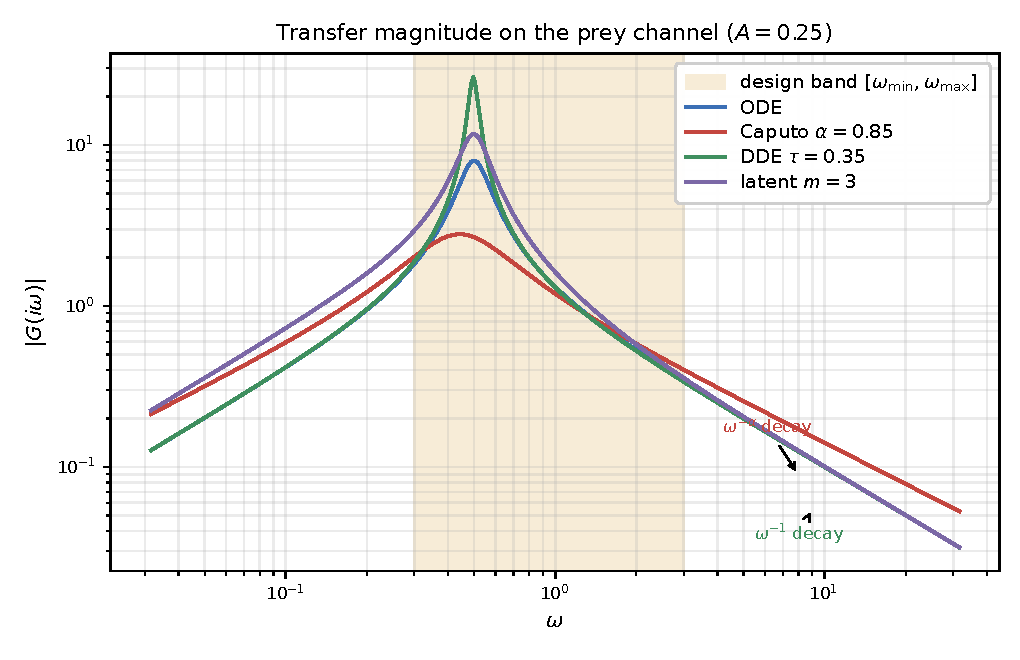
\includegraphics[width=0.75\textwidth]{fig01_transfer_magnitude}
\caption{$|G(i\omega)|$ on the prey channel at $A=0.25$ for ODE, Caputo ($\alpha=0.85$), DDE ($\tau=0.35$), and latent ($m=3$). The Caputo curve separates over the design band and approaches its $O(\omega^{-\alpha})$ decay.}
\label{fig:transfer-mag}
\end{figure}

\begin{figure}[htbp]\centering
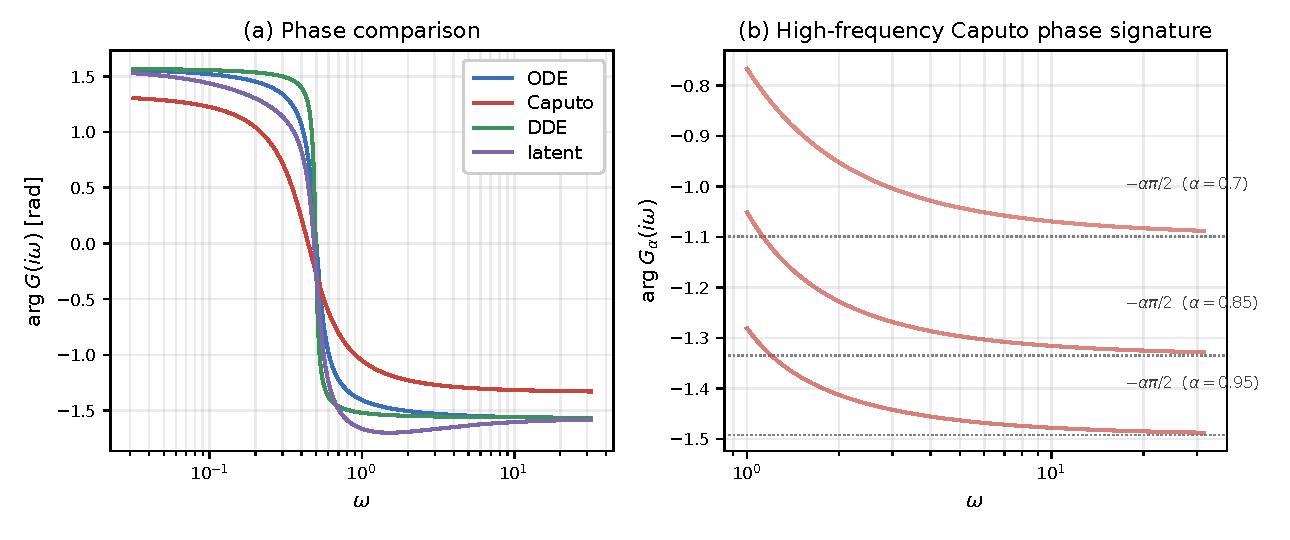
\includegraphics[width=0.90\textwidth]{fig02_phase_2panel}
\caption{Phase on the prey channel. Left: the four mechanisms across frequency. Right: convergence of the Caputo phase to the asymptote $-\alpha\pi/2$, independent of scale.}
\label{fig:transfer-phase}
\end{figure}

\subsection{From exact signatures to finite-horizon ambiguity}
The two panels must be read jointly with Theorem~\ref{thm:T9b}. The $O(\omega^{-\alpha})$ decay and the $-\alpha\pi/2$ phase identify the Caputo channel asymptotically, but an experiment observes a finite band $[\omega_{\min},\omega_{\max}]$, a finite window $[0,T]$, and noise of level $\sigma$. On that restricted set a latent model with enough modes matches the observable part of the response while remaining analytically distinct --- the coexistence of exact separation (Theorem~\ref{thm:T4}) and finite-horizon mimicry (Theorem~\ref{thm:T9b}) stated in frequency-domain terms.

The prey-response computation restates the point in the instrumented channel. Table~\ref{tab:state-approx} lists the certified $L^1$ bounds $\widehat E_m^{\rm state}$ and the induced testing floors at $\alpha=0.85$, $T=12$, $\sigma=0.10$: from $m=4$ to $m=32$ the enclosure shrinks by a factor of $77$ (from $0.5334$ to $0.0069$ at $A=0.25$) and the testing bound rises from $0.374$ to $0.498$, i.e., to within $0.002$ of the equal-prior chance level. Two bounds are reported. Since the two hypotheses are Gaussian with common covariance $\sigma^2I$, the exact minimax error $\Phi(-d/2)$ with $d=\|\Delta\mu\|_2/\sigma$ is available and is uniformly tighter than the Pinsker bound; the difference matters only at small $m$, where Pinsker understates the floor by $0.034$ at $m=4$. We quote the exact bound and retain Pinsker for comparability with the literature.

\begin{table}[htbp]
\centering
\caption{Certified finite-state approximation of the fractional prey response and induced testing lower bounds at $\alpha=0.85$, $T=12$, pulse $\|u\|_2\le0.120$, and $\sigma=0.10$. The exact bound is $\Phi(-d/2)$ with $d=\|\Delta\mu\|_2/\sigma$, valid because the two hypotheses share the covariance $\sigma^2I$; Pinsker is reported for comparison and is uniformly looser.}
\label{tab:state-approx}
\small
\begin{tabular}{ccccccc}
\hline
& \multicolumn{3}{c}{$A=0.25$} & \multicolumn{3}{c}{$A=0.30$}\\
$m$ & $\widehat E_m^{\rm state}$ & $P_e^*$ (exact) & $P_e^*$ (Pinsker) & $\widehat E_m^{\rm state}$ & $P_e^*$ (exact) & $P_e^*$ (Pinsker)\\
\hline
4  & 0.5334 & 0.3745 & 0.340 & 0.4706 & 0.3888 & 0.359\\
8  & 0.1254 & 0.4700 & 0.462 & 0.0898 & 0.4785 & 0.473\\
16 & 0.0273 & 0.4935 & 0.492 & 0.0204 & 0.4951 & 0.494\\
32 & 0.0069 & 0.4983 & 0.498 & 0.0066 & 0.4984 & 0.498\\
\hline
\end{tabular}
\end{table}

Because Table~\ref{tab:state-approx} stops at $m=32$ it shows only part of the obstruction. Table~\ref{tab:state-approx-large} continues it to $m=128$ using an explicit positive-weight exponential-sum surrogate constructed as in Lemma~\ref{thm:T9b} rather than the interval-optimised class $\mathcal G_m$. Because that surrogate is one admissible element and not the infimum, its error exceeds $\widehat E_m^{\rm state}$ --- by factors $2.4$ at $m=4$ and $3.3$ at $m=32$ where the two overlap --- so the induced floors are valid and conservative. They reach $0.4996$ at $m=64$ and $0.49999$ at $m=128$: at attainable latent orders the finite-state rival is indistinguishable from the fractional model under this protocol, and no experiment restricted to the declared budget can separate them.

\begin{table}[htbp]
\centering
\caption{Prey-response $L^1$ error of an explicit positive-weight exponential-sum surrogate (not the certified infimum, hence an upper bound on $\widehat E_m^{\rm state}$) and the induced exact testing floor, $\alpha=0.85$, $A=0.25$, $T=12$, $\|u\|_2\le0.120$, $\sigma=0.10$.}
\label{tab:state-approx-large}
\small
\begin{tabular}{cccc}
\hline
$m$ & $\|g_\alpha-g_m\|_{L^1(0,T)}$ & quadrature error & $P_e^*$ (exact)\\
\hline
4   & $1.29\cdot10^{0}$   & $2.1\cdot10^{-7}$ & 0.2202\\
8   & $4.98\cdot10^{-1}$  & $1.0\cdot10^{-7}$ & 0.3827\\
16  & $1.30\cdot10^{-1}$  & $7.6\cdot10^{-9}$ & 0.4689\\
32  & $2.31\cdot10^{-2}$  & $3.0\cdot10^{-8}$ & 0.4945\\
64  & $1.58\cdot10^{-3}$  & $2.1\cdot10^{-8}$ & 0.4996\\
128 & $4.83\cdot10^{-5}$  & $6.3\cdot10^{-9}$ & 0.49999\\
\hline
\end{tabular}
\end{table}

The table is one-sided. A large lower bound on $P_e^*$ proves that the specified experiment cannot reliably separate $g_\alpha$ from at least one admitted rival $g_m$; a small bound proves nothing in the converse direction, so such cells are inconclusive rather than certified-easy. Figure~\ref{fig:atlas} applies this reading across $(\alpha,A,m)$: cells outside the focal Matignon-stable regime ($\alpha>\alpha^*(A)$) are hatched and excluded from the headline interpretation.

\begin{figure}[htbp]\centering
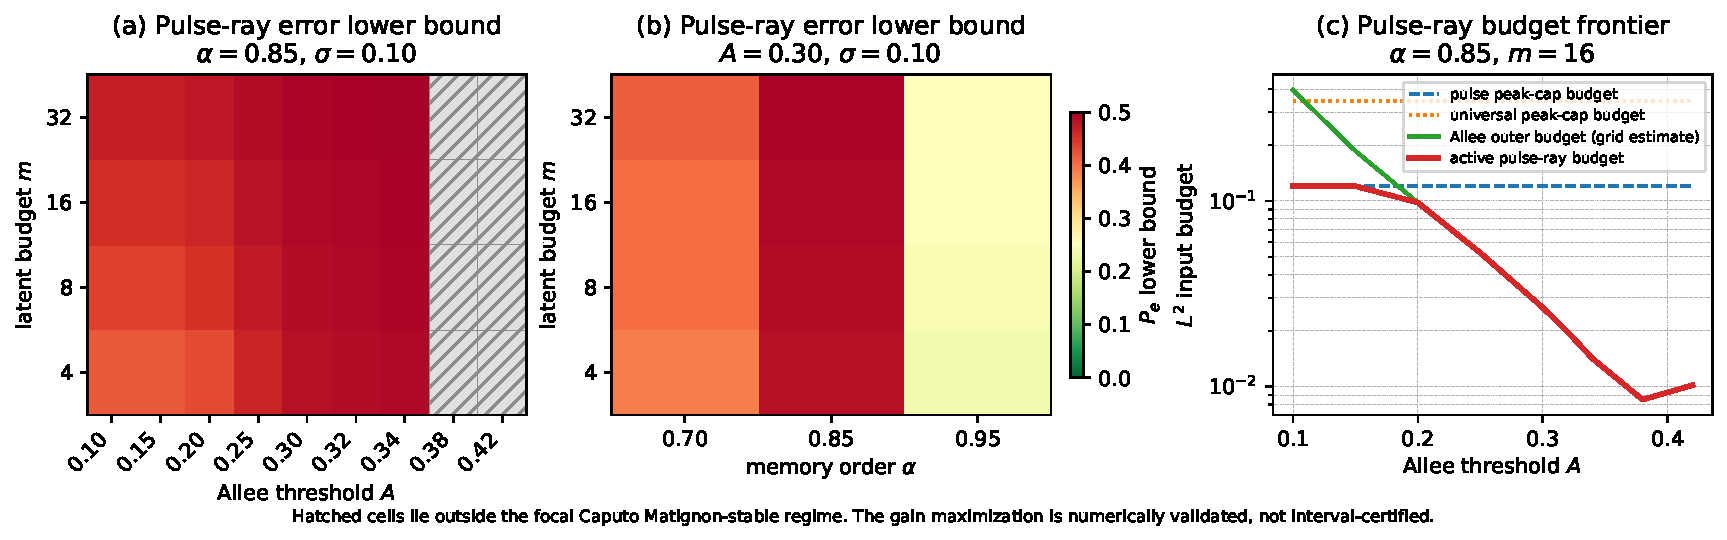
\includegraphics[width=0.92\textwidth]{fig18_safe_discrimination_atlas}
\caption{Protocol-restricted discrimination atlas over $(\alpha,A,m)$: lower bound on the model-selection error under the declared pulse protocol. The bound increases with latent budget $m$ and toward weakly separated regimes; hatched cells violate the Matignon condition $\alpha<\alpha^*(A)$ and are excluded from stable-regime conclusions.}
\label{fig:atlas}
\end{figure}

\section{Fractional-Delay Model: Dedicated Simulation Study}
\label{sec:fd}

Sections~\ref{sec:analysis}--\ref{sec:response} treated fractional memory and explicit delay as competing hypotheses. This section studies the mechanism carrying both, via the combined model~\eqref{eq:fdmodel}. Its boundaries coincide with the two mechanisms already characterized: $\tau=0$ is the pure Caputo model and $\alpha=1$ is the DDE benchmark, with both limits verified to the tolerances of Table~\ref{tab:solver-validation}. The interior of $(\alpha,\tau)\in[0.70,1]\times[0,0.5]$ then measures whether the two effects reinforce, cancel, or generate responses outside the reach of either pure explanation.

The scope is deliberately limited: no general theory of fractional delay equations is attempted. The study is a stress test of the discrimination framework under identical conditions to the rest of the paper --- same ecology, same prey channel, same budget $\|u\|_\infty\le0.10$, same observables --- with only $(\alpha,\tau)$ varying. What it exposes is invisible to pairwise comparisons: when a system carries a hereditary response \emph{and} a physiological lag, a binary ``fractional versus delay'' classification is misspecified even if each limiting model fits part of the data.

\subsection{Transient trajectories}
Figure~\ref{fig:fdtraj} fixes $A=0.25$, $\alpha=0.85$, applies the identical prey pulse, and varies $\tau\in\{0,0.15,0.35,0.50\}$. The prey trajectory changes little; the predator response shifts visibly with $\tau$ and its late transient becomes increasingly delay-sensitive. All four trajectories satisfy $x(t)>A$ throughout, with minimum margin $\ge0.356$ (Table~\ref{tab:fd-bridge-cells}).

\begin{figure}[htbp]\centering
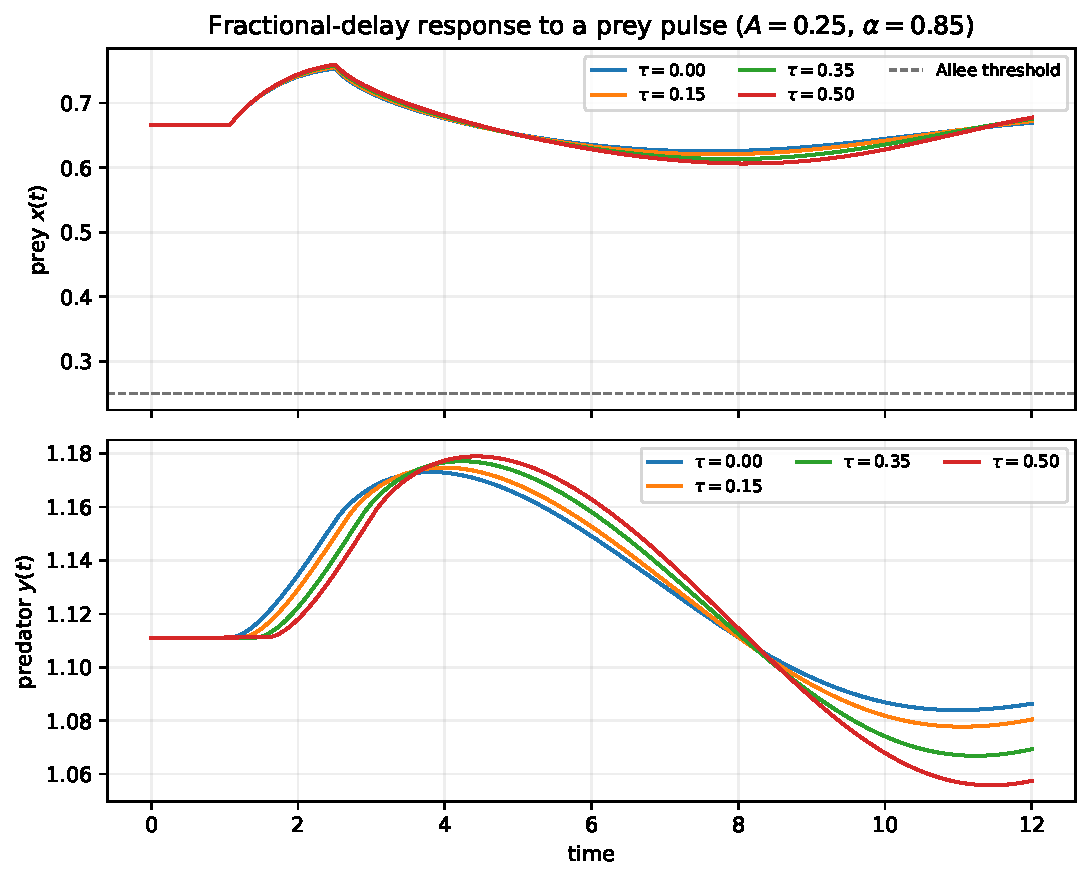
\includegraphics[width=0.82\textwidth]{fig20_fractional_delay_trajectories}
\caption{Combined fractional-delay response to the same prey pulse at $A=0.25$ and $\alpha=0.85$. Increasing delay shifts the predator response and reshapes the late transient while the fractional-memory relaxation pattern persists.}
\label{fig:fdtraj}
\end{figure}

\subsection{Fractional-order/delay parameter plane}
Figure~\ref{fig:fdbridge} maps the $7\times6$ grid $\alpha\in\{0.70,\ldots,1.00\}$, $\tau\in\{0,\ldots,0.50\}$. The edge $\tau=0$ has zero distance to the pure Caputo model and the edge $\alpha=1$ zero distance to the DDE, by construction; the quantity of interest is the interior escape rate from both. The right panel adds the safety dimension: a delay that leaves the margin nearly untouched at $\alpha=0.75$ (from $0.3917$ to $0.3850$ over $\tau\in[0.1,0.5]$) removes $21\%$ of it at $\alpha=0.95$ (from $0.3345$ to $0.2629$).

\begin{figure}[htbp]\centering
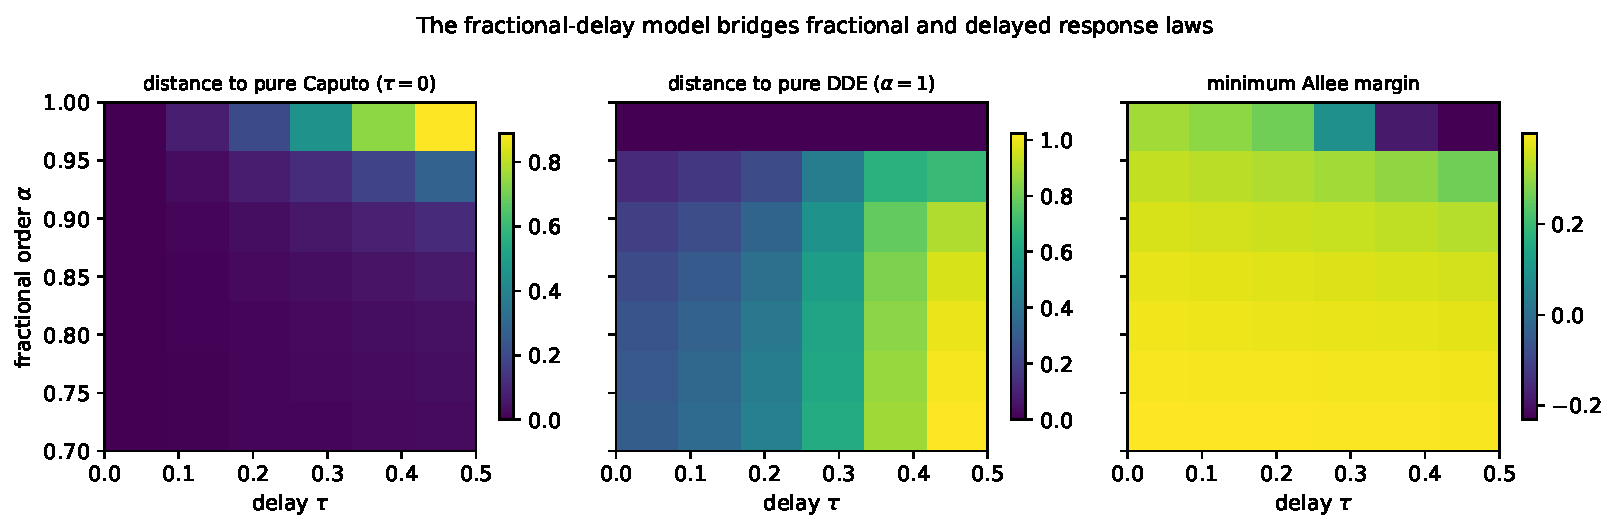
\includegraphics[width=0.98\textwidth]{fig21_fractional_delay_bridge}
\caption{Fractional-delay bridge over $(\alpha,\tau)$. Left: trajectory distance to the pure Caputo limit. Center: distance to the pure DDE limit. Right: minimum Allee margin under the same pulse. Parts of the interior are poorly represented by either limit alone.}
\label{fig:fdbridge}
\end{figure}

Table~\ref{tab:fd-bridge-cells} lists nine representative cells. For each fixed $\alpha$, $d_{\rm Caputo}$ increases monotonically in $\tau$ while $d_{\rm DDE}$ remains large ($\ge0.16$ in every displayed cell). The steepest row is $\alpha=0.95$: $d_{\rm Caputo}$ grows by a factor of $9.4$ (from $0.0299$ at $\tau=0.10$ to $0.2805$ at $\tau=0.50$) while the minimum margin falls from $0.3345$ to $0.2629$. In this corner of parameter space, added delay increases identifiability and ecological risk simultaneously.

\begin{table}[htbp]
\centering
\caption{Representative cells from the fractional-delay bridge at $A=0.25$ under the pulse experiment. Distances are trajectory $L^2$ distances to the corresponding limiting models.}
\label{tab:fd-bridge-cells}
\small
\begin{tabular}{ccccc}
\hline
$\alpha$ & $\tau$ & distance to Caputo & distance to DDE & min. $[x(t)-A]$\\
\hline
0.75 & 0.10 & 0.0063 & 0.3426 & 0.3917\\
0.75 & 0.30 & 0.0182 & 0.6145 & 0.3887\\
0.75 & 0.50 & 0.0315 & 1.0086 & 0.3850\\
0.85 & 0.10 & 0.0103 & 0.2900 & 0.3724\\
0.85 & 0.30 & 0.0334 & 0.5683 & 0.3655\\
0.85 & 0.50 & 0.0625 & 0.9606 & 0.3566\\
0.95 & 0.10 & 0.0299 & 0.1645 & 0.3345\\
0.95 & 0.30 & 0.1142 & 0.4330 & 0.3123\\
0.95 & 0.50 & 0.2805 & 0.6875 & 0.2629\\
\hline
\end{tabular}
\end{table}

\subsection{Which input exposes the combined mechanism?}
Each input is scored over the nine cells $\alpha\in\{0.75,0.85,0.95\}\times\tau\in\{0.15,0.30,0.45\}$ by the mean of $\min(d_{\rm Caputo},d_{\rm DDE})$; the $\min$ penalizes inputs that separate the combined response from only one limit. Results (Figure~\ref{fig:fddesign}, Table~\ref{tab:fd-design-ranking}): multisine attains the highest score ($0.1332$) with crossing fraction $1/3$; PRBS ($0.0909$), sinusoid ($0.0894$), and chirp ($0.0861$) cross in all nine cells; pulse ($0.0627$) and multiscale ($0.0338$) never cross but discriminate weakly. The safety--informativeness tension of Section~\ref{sec:benchmark} reappears unchanged in the two-memory model.

\begin{table}[htbp]
\centering
\caption{Fractional-delay design stress test at $A=0.25$. The score averages the minimum distance to the Caputo and DDE limits over $\alpha\in\{0.75,0.85,0.95\}$ and $\tau\in\{0.15,0.30,0.45\}$.}
\label{tab:fd-design-ranking}
\small
\begin{tabular}{lccc}
\hline
\textbf{Input} & \textbf{mean bridge score} & \textbf{worst Allee margin} & \textbf{crossing fraction}\\
\hline
multisine  & 0.1332 & -0.2103 & 0.333\\
PRBS       & 0.0909 & -0.2814 & 1.000\\
sinusoid   & 0.0894 & -0.2777 & 1.000\\
chirp      & 0.0861 & -0.2763 & 1.000\\
pulse      & 0.0627 &  0.2770 & 0.000\\
multiscale & 0.0338 &  0.3171 & 0.000\\
\hline
\end{tabular}
\end{table}

\begin{figure}[htbp]\centering
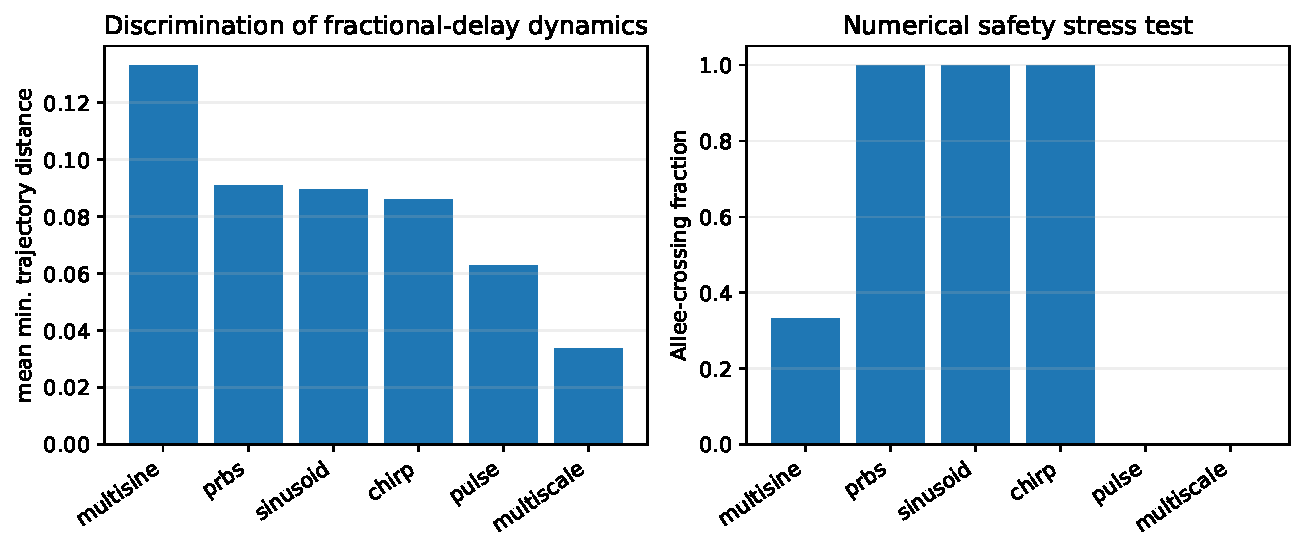
\includegraphics[width=0.86\textwidth]{fig22_fractional_delay_design_ranking}
\caption{Input-design stress test for fractional-delay dynamics. Left: mean minimum trajectory distance from the two limiting explanations (pure Caputo and pure DDE). Right: numerical Allee-crossing fraction on the same $(\alpha,\tau)$ grid. Broadband inputs expose the combined mechanism more strongly and are substantially less safe.}
\label{fig:fddesign}
\end{figure}

\subsection{Delay sweep}
Figure~\ref{fig:fdsweep} sweeps $\tau\in[0,0.55]$ at twelve points for $\alpha\in\{0.75,0.85,0.95\}$. In all three orders the predator peak time increases with $\tau$, its amplitude grows moderately (by $<1\%$), and the minimum Allee margin decreases --- weakly at $\alpha=0.75$, strongly at $\alpha=0.95$. Delay is thus observable as a reproducible timing shift, not merely as a fitting parameter, and the shift carries a quantifiable safety cost.

Endpoints (Table~\ref{tab:fd-delay-summary}): at $\alpha=0.85$, the change $\tau:0\to0.55$ moves the predator peak from $t=3.814$ to $t=4.500$ ($+0.686$) and the margin from $0.3759$ to $0.3548$ ($-5.6\%$); at $\alpha=0.95$ the same change moves the peak from $t=4.157$ to $t=4.886$ and the margin from $0.3434$ to $0.2384$ ($-30.6\%$).

\begin{table}[htbp]
\centering
\caption{Endpoint summary of the delay sweep under the pulse experiment. Values compare $\tau=0$ with $\tau=0.55$.}
\label{tab:fd-delay-summary}
\small
\begin{tabular}{cccccc}
\hline
$\alpha$ & $\tau$ & predator peak time & predator peak & min. Allee margin\\
\hline
0.75 & 0    & 3.343 & 1.1634 & 0.3934\\
0.75 & 0.55 & 4.029 & 1.1681 & 0.3843\\
0.85 & 0    & 3.814 & 1.1724 & 0.3759\\
0.85 & 0.55 & 4.500 & 1.1788 & 0.3548\\
0.95 & 0    & 4.157 & 1.1838 & 0.3434\\
0.95 & 0.55 & 4.886 & 1.1925 & 0.2384\\
\hline
\end{tabular}
\end{table}

The sampling-design implication is direct. Delay is expressed in the timing of the predator peak (at $t\approx3.3$--$4.9$ across the tested grid); fractional memory in the relaxation tail beyond it. A window restricted to the initial prey perturbation misses both signatures: it ends before the delayed predator response and far before the tail. Dense sampling around the predicted peak, extended through the tail, captures both --- the recommendation quantified in Section~\ref{sec:prospect}.

\begin{figure}[htbp]\centering
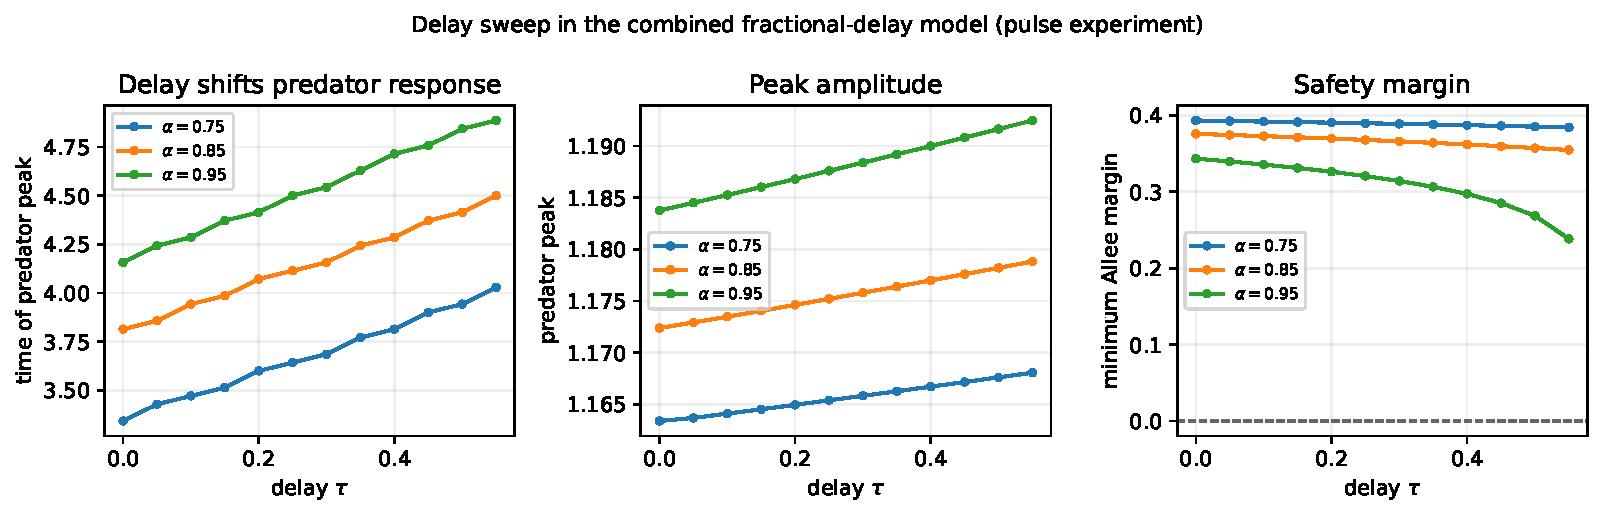
\includegraphics[width=0.98\textwidth]{fig23_fractional_delay_sweep}
\caption{Delay sweep under the pulse experiment. The predator peak arrives later as $\tau$ grows, its amplitude increases moderately, and the numerical Allee margin shrinks --- consistently across the three displayed fractional orders.}
\label{fig:fdsweep}
\end{figure}

\section{Experiment Design and Safety}
\label{sec:design}

The design theory itself is classical in outline; we state just enough here to motivate the waveforms, and refer the full development with proofs to the Supplementary Material. For two Gaussian linearized models with common covariance, the pairwise information carried by an input $u$ takes the quadratic form
\[
D_{ij}(u)=\frac12\langle u,Q_{ij}u\rangle,
\]
so under the energy constraint $\|u\|^2\le E$ the optimum is the leading eigenfunction of $Q_{ij}$, and the robust frequency-domain problem admits an optimum with finite frequency support (both proved in the Supplementary Material). These two facts justify restricting the search to the six implementable waveform families of Figure~\ref{fig:waveforms} instead of an infinite-dimensional input space.

\begin{figure}[htbp]\centering
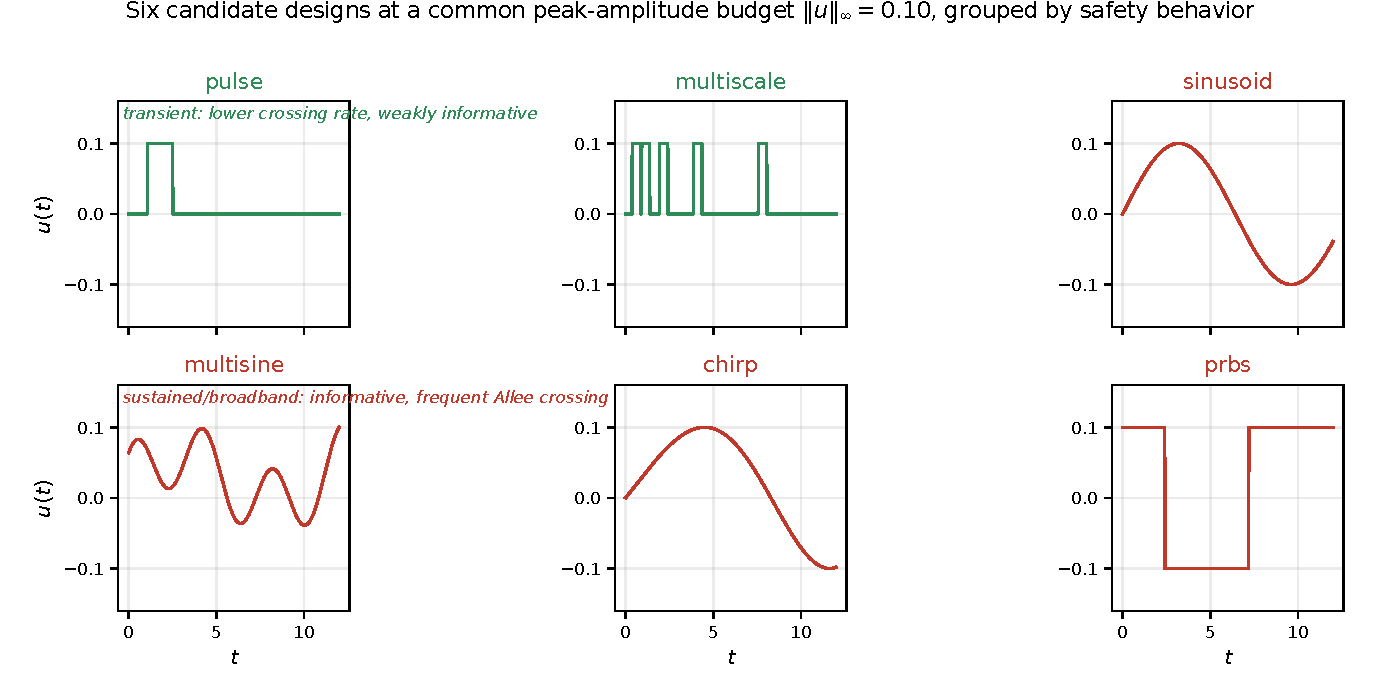
\includegraphics[width=0.95\textwidth]{fig04_waveforms}
\caption{Six candidate perturbations at the common peak-amplitude budget. Transient and broadband designs interrogate the memory law in different ways --- and behave very differently with respect to safety once the nonlinear simulations run.}
\label{fig:waveforms}
\end{figure}

\begin{figure}[htbp]\centering
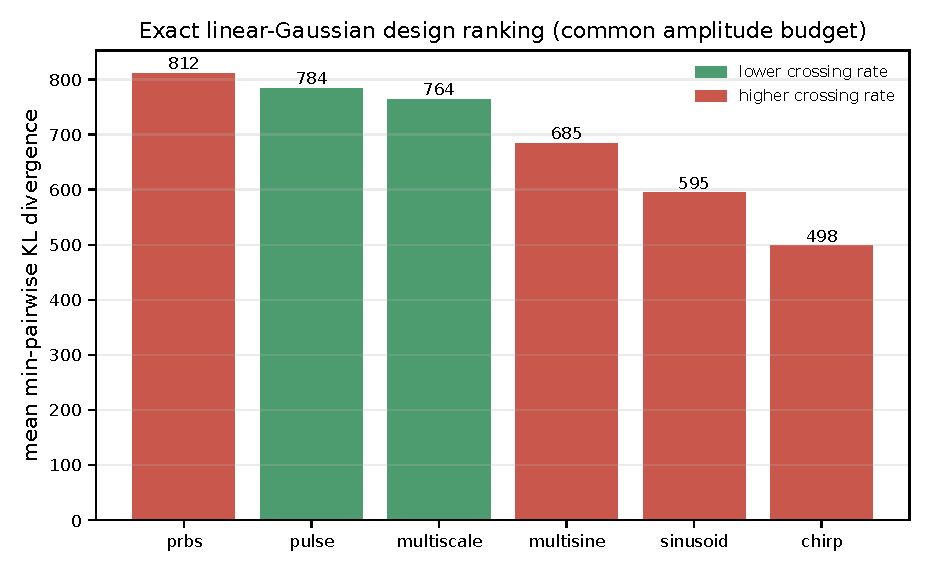
\includegraphics[width=0.68\textwidth]{fig05_linear_ranking}
\caption{Linear-Gaussian design ranking by mean minimum pairwise KL divergence. Nonlinear state safety is invisible at this level, so the ranking serves as an information benchmark, not as a final experimental recommendation.}
\label{fig:linear-ranking}
\end{figure}

\subsection{Strong-Allee safety}
The one-sided Allee constraint requires $x(t)>A+\eta$ for all $t\in[0,T]$. For the linearized system, a sufficient pulse-amplitude envelope follows from the prey impulse gain; for the nonlinear system, the strict inward-pointing rectangle theorem and its four face inequalities are given in the Supplementary Material. One structural point belongs in the main text: state safety alone does \emph{not} bound input energy. A stable strictly proper channel attenuates high frequencies as $O(\omega^{-1})$ or faster, so an oscillatory input of arbitrarily large $\|u\|_2$ can leave the state nearly unmoved. Every quantitative testing bound in this paper is therefore tied to an explicit actuator or protocol class --- here, the declared peak-amplitude pulse budget $\|u\|_\infty\le0.10$, $\|u\|_2\le0.120$.

\begin{figure}[htbp]\centering
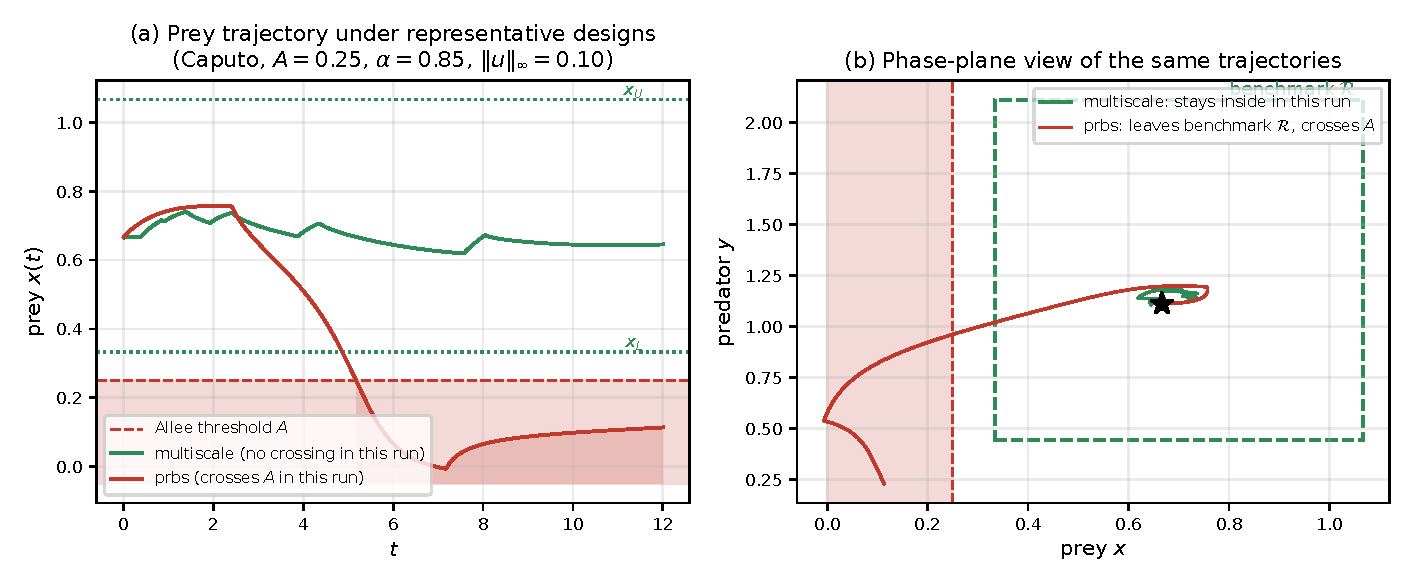
\includegraphics[width=0.92\textwidth]{fig15_safety_geometry}
\caption{Representative nonlinear safety geometry. In the run shown, a multiscale transient stays above the Allee threshold while PRBS crosses it. The rectangle drawn is a benchmark diagnostic region; rigorous positive invariance requires the strict face conditions stated in the Supplementary Material.}
\label{fig:safety-geometry}
\end{figure}

\section{Large-Scale Model-Discrimination Benchmark}
\label{sec:benchmark}

The benchmark compares ODE, Caputo, retarded DDE, and latent-$3$ mechanisms at matched operating conditions. The primary stable-regime task uses $A\in\{0.20,0.25\}$; a separate task at $A>2/7$ addresses the easier stability-verdict question. The decision rule is BIC throughout --- an information criterion, not Bayesian model evidence, and it is reported as such.

\subsection{Benchmark design and decision rule}
The benchmark is not organized around any single synthetic trajectory. It asks whether the qualitative design conclusions survive joint variation of memory strength ($\alpha$), observation noise (three SNR levels), observation channel (three), and waveform (six families). For each generated trajectory, all four candidates are fitted under one observation protocol and compared by BIC; the object under evaluation is a reproducible decision rule.

Two factorial layers are kept separate. The nonlinear stable-regime benchmark has 1512 cells $\times$ 200 stochastic replicates (302{,}400 trajectories, zero solver divergences); a linear-Gaussian factorial of 1458 cells serves only as an information-ranking reference (Figure~\ref{fig:linear-ranking}). The layers can disagree: the linear ranking measures local operator separation, while the nonlinear layer sees the Allee geometry, and an input that tops the linear ranking is disqualified once its trajectories cross $x=A$ (Table~\ref{tab:benchmark-safety}).

Macro-averaged accuracy in the primary four-class stable task is $0.537$ versus chance $0.25$. By input family:
\[
\begin{aligned}
\text{PRBS }(0.584)&\approx\text{ multisine }(0.583)>\text{sinusoid }(0.534),\\
&>\text{chirp }(0.507)>\text{pulse }(0.414)>\text{multiscale }(0.324).
\end{aligned}
\]
Difficulty is dominated by two axes (Table~\ref{tab:benchmark-stratified}). As $\alpha\to1$ the mechanisms converge and accuracy falls from $0.702$ ($\alpha=0.70$) to $0.312$ ($\alpha=0.95$); across noise, accuracy is $0.756$/$0.444$/$0.273$ at high/medium/low SNR. The channel effect is smaller: both-species observation attains $0.530$, prey-only $0.516$ (the directly actuated channel remains structurally sufficient), predator-only $0.427$.

\begin{table}[htbp]
\centering
\caption{Stable-regime four-class BIC accuracy stratified by fractional order, SNR, and observation channel.}
\label{tab:benchmark-stratified}
\footnotesize
\setlength{\tabcolsep}{4pt}
\begin{tabular}{llc@{\quad}llc}
\hline
\textbf{Axis} & \textbf{level} & \textbf{accuracy} & \textbf{Axis} & \textbf{level} & \textbf{accuracy}\\
\hline
$\alpha$ & 0.70 & 0.702 & SNR & high & 0.756\\
          & 0.85 & 0.557 &     & medium & 0.444\\
          & 0.90 & 0.467 &     & low & 0.273\\
          & 0.95 & 0.312 & channel & prey & 0.516\\
          &      &       &         & predator & 0.427\\
          &      &       &         & both & 0.530\\
\hline
\end{tabular}
\end{table}

Class-wise statistics refine the picture (Figure~\ref{fig:confusion}). ODE: recall $0.972$, precision $0.227$ --- under weak excitation the subtler mechanisms are absorbed into the simplest class. Caputo: recall $0.524$, precision $0.984$ --- a Caputo verdict, once issued, is nearly always correct. DDE: $0.410/0.731$; latent-$3$: $0.242/0.848$. The dominant failure mode is therefore conservative collapse toward the simpler explanation when the data underdetermine the memory law, not symmetric confusion among mechanisms.

\begin{figure}[htbp]\centering
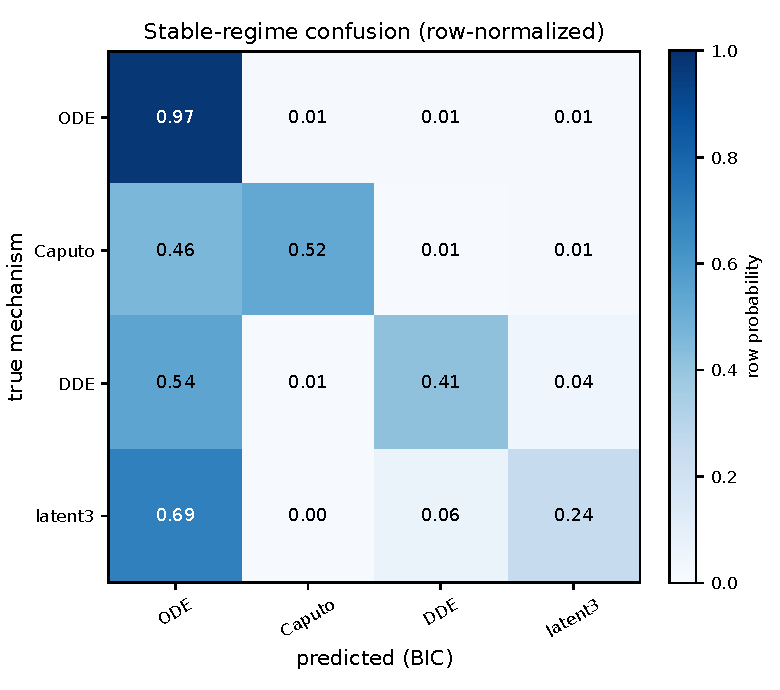
\includegraphics[width=0.56\textwidth]{fig07_confusion}
\caption{Row-normalized confusion matrix for the stable four-class task. Under weak excitation the simplest ODE mechanism absorbs the rest; Caputo predictions, when made, are highly precise.}
\label{fig:confusion}
\end{figure}

\begin{figure}[htbp]\centering
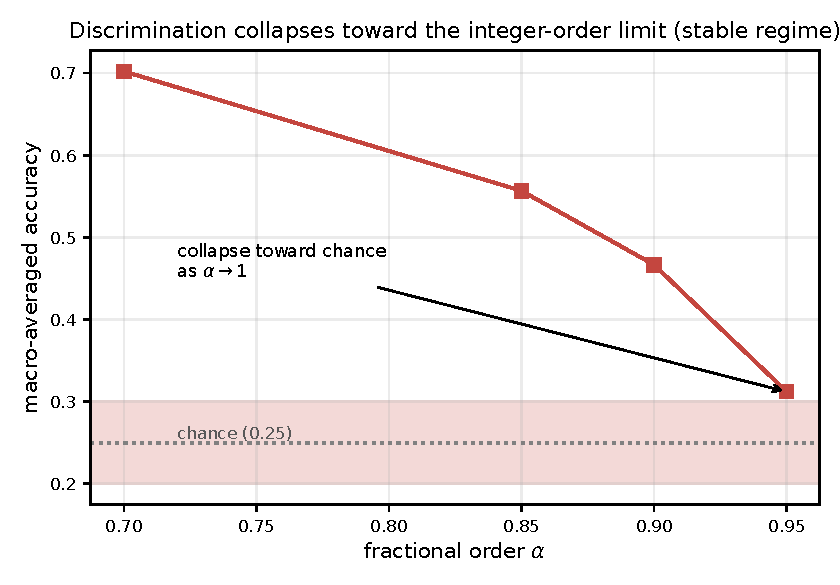
\includegraphics[width=0.58\textwidth]{fig08_accuracy_vs_alpha}
\caption{Model-selection accuracy versus fractional order. The closer $\alpha$ gets to the integer-order limit, the harder the memory mechanisms are to tell apart.}
\label{fig:acc-alpha}
\end{figure}

\begin{figure}[htbp]\centering
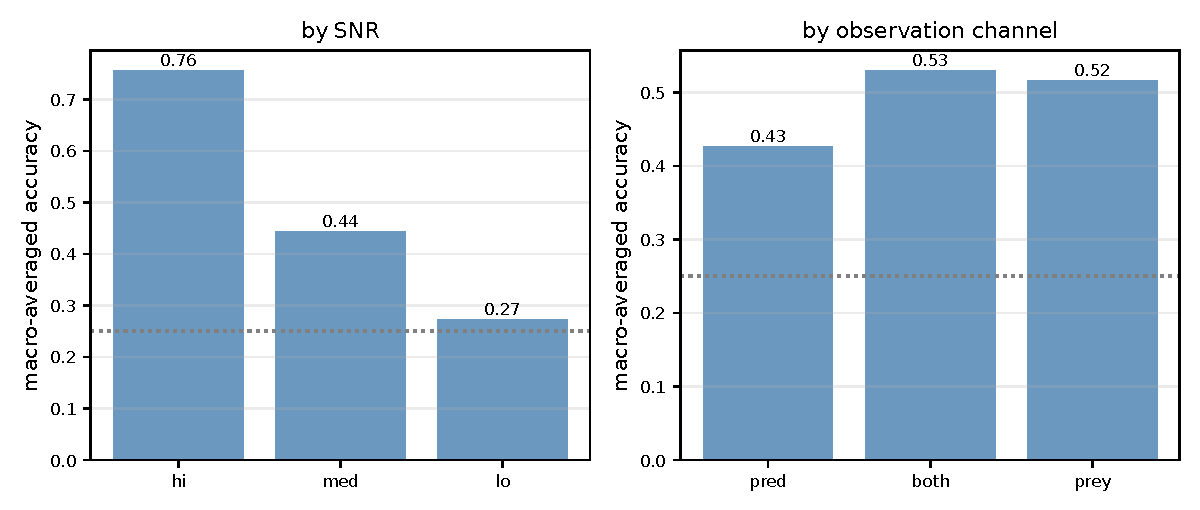
\includegraphics[width=0.82\textwidth]{fig09_accuracy_snr_channel}
\caption{Accuracy stratified by SNR and observation channel. The benchmark is strongly noise-limited; observing both species gives the best average accuracy.}
\label{fig:acc-snr}
\end{figure}

\subsection{Safety--informativeness trade-off}
Numerical state safety is reported on its own axis, never folded into the information score. At the common budget $\|u\|_\infty\le0.10$: multiscale never crosses the threshold (rate $0.000$) and discriminates worst ($0.324$); PRBS and sinusoid discriminate best ($0.584$, $0.534$) and cross at rates $1.000$; multisine matches PRBS in accuracy ($0.583$) at crossing rate $0.357$.

Table~\ref{tab:benchmark-safety} gives the frontier. Multiscale retains a positive minimum margin of $0.292$ at the lowest accuracy; the pulse is the practical compromise, crossing at rate $0.071$ with accuracy $0.414$ --- below the broadband designs by $0.17$.

\begin{table}[htbp]
\centering
\caption{Nonlinear stable-benchmark trade-off at the common peak-amplitude budget. Safety values are numerical benchmark diagnostics, not invariant-set certificates.}
\label{tab:benchmark-safety}
\footnotesize
\begin{tabular}{lccc}
\hline
\textbf{Input} & \shortstack{\textbf{macro}\\\textbf{accuracy}} & \shortstack{\textbf{Allee}\\\textbf{crossing rate}} & \shortstack{\textbf{minimum}\\\textbf{Allee margin}}\\
\hline
PRBS       & 0.584 & 1.000 & -0.3139\\
multisine  & 0.583 & 0.357 & -0.2405\\
sinusoid   & 0.534 & 1.000 & -0.3058\\
chirp      & 0.507 & 0.929 & -0.3012\\
pulse      & 0.414 & 0.071 & -0.1207\\
multiscale & 0.324 & 0.000 &  0.2921\\
\hline
\end{tabular}
\end{table}

The table also fixes a methodological point: the linear-Gaussian ranking alone cannot select the final experiment. Linear theory scores an input by operator separation; the nonlinear ecology can answer the same input by leaving the coexistence basin, after which no local identification experiment remains. Safety must be evaluated on the nonlinear state trajectory, not extrapolated from the linear information score.

\begin{figure}[htbp]\centering
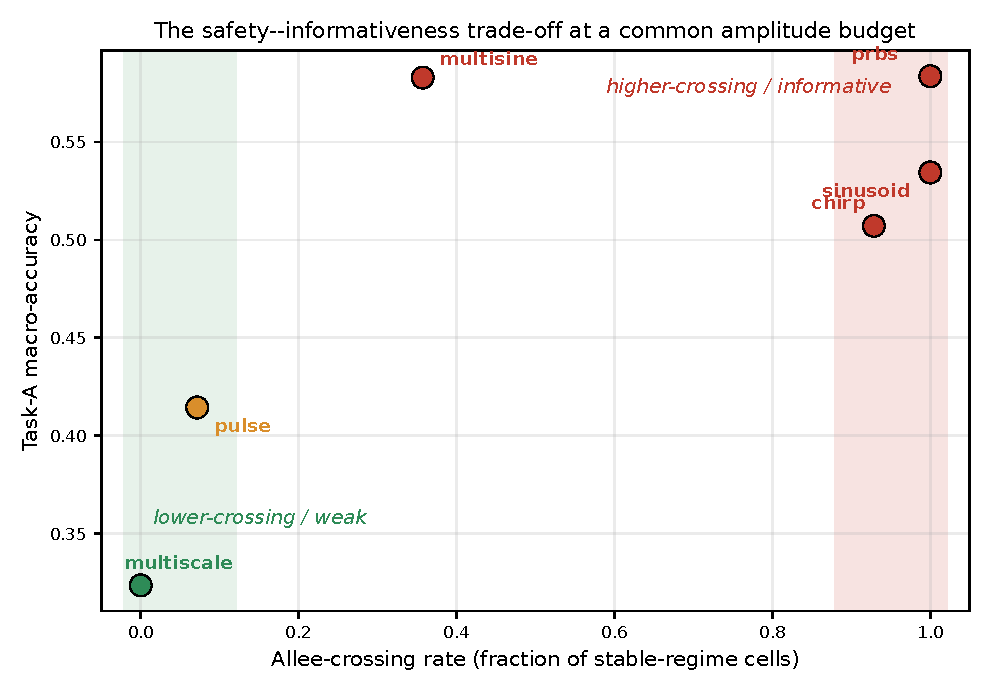
\includegraphics[width=0.72\textwidth]{fig10_safety_tradeoff}
\caption{Headline benchmark trade-off. Broadband and sustained designs climb in discrimination but drift toward higher Allee-crossing rates; transient designs stay in the low-crossing, less-informative corner.}
\label{fig:safety-tradeoff}
\end{figure}

\section{Prospective Experimental Interpretation}
\label{sec:prospect}

Laboratory predator--prey microcosms provide the controlled perturbation setting the simulations presume~\cite{E10,E11,E12}, and the numerical results translate into specific protocol constraints. A first experiment should operate in a stable strong-Allee regime ($A\le2/7$), apply a bounded prey perturbation ($\|u\|_\infty\le0.10$ in normalized units), observe both populations where instrumentation allows (accuracy $0.530$ versus $0.516$ prey-only; Table~\ref{tab:benchmark-stratified}), and postpone broadband excitation until a transient probe has established the available margin.

The fractional-delay study adds one operational diagnostic. Delay moves the predator peak time (by up to $+0.73$ time units over $\tau\in[0,0.55]$; Table~\ref{tab:fd-delay-summary}); fractional order reshapes the long transient and phase. A scheme sampling densely around the predicted peak ($t\approx3.3$--$4.9$ on the tested grid) and recording through the relaxation tail resolves both signatures; uniform sparse sampling can miss both.

A Bayesian sequential layer is specified in the Supplementary Material and deliberately not executed; the evidence in the main text is limited to deterministic solvers, interval enclosures, and BIC benchmarks, all rerunnable from the released scripts.

\subsection*{A two-stage prospective protocol}
The observed frontier (Tables~\ref{tab:benchmark-safety} and~\ref{tab:fd-design-ranking}) argues against applying the most informative perturbation first. Stage~1 uses a transient input with low observed crossing rate (pulse, $0.071$; multiscale, $0.000$) to estimate the local response scale and verify a comfortable margin above $A$. Stage~2 is conditional: multisine-type excitation (accuracy $0.583$, crossing rate $0.357$) is applied only if Stage~1 leaves adequate margin. No Bayes-optimality is claimed for this sequencing; it is a direct reading of the frontier, summarized in Table~\ref{tab:prospective-protocol}.

\begin{table}[htbp]
\centering
\caption{Prospective microcosm workflow suggested by the simulation results.}
\label{tab:prospective-protocol}
\footnotesize
\setlength{\tabcolsep}{3pt}
\begin{tabular}{p{0.10\textwidth}p{0.22\textwidth}p{0.27\textwidth}p{0.25\textwidth}}
\hline
\textbf{Stage} & \textbf{Perturbation} & \textbf{Primary measurements} & \textbf{Decision / purpose}\\
\hline
0 & no perturbation & baseline prey/predator variability & estimate noise and confirm operating point\\
1 & pulse or multiscale & dense early prey observations; predator peak timing; minimum prey level & verify local response and available safety margin\\
2 & multisine if margin permits & both species over the full transient and relaxation tail & maximize separation of memory mechanisms\\
3 & optional repeat / altered horizon & same channels, replicated under matched conditions & test robustness of the selected mechanism and estimate variability\\
\hline
\end{tabular}
\end{table}

Three measurement priorities follow from the simulations. (i) The actuated prey channel carries the strongest early signal: sample densely immediately after the perturbation. (ii) The delayed pathway is expressed in predator-peak timing: concentrate observations near the anticipated peak rather than uniformly. (iii) Fractional memory dominates the slow relaxation tail: extend the horizon well past the peak. The resulting design is nonuniform --- dense around the forcing and the peak, sparser but longer through relaxation.

On units: the simulations are dimensionless with a normalized budget. A physical implementation must map state and input to organism counts, biomass, or resource-manipulation units and must fix an operational margin above the \emph{empirical} Allee threshold. This calibration is application-specific and is not inferred from simulation here.

\section{Discussion}
\label{sec:discussion}

Three conclusions are supported consistently by the analytical results of Section~\ref{sec:analysis} and the numerical layers of Sections~\ref{sec:response}--\ref{sec:benchmark}.

First, \emph{structural identifiability and practical discrimination are different questions}. The Caputo transfer carries an exact $O(\omega^{-\alpha})$ signature (Theorem~\ref{thm:T4}); finite latent models approximate the same response to any tolerance on $[0,T]$ (Corollary~\ref{cor:closure}); and the testing bounds quantify the gap --- $P_e^*\ge0.498$ at $m=32$ under the pulse protocol (Table~\ref{tab:state-approx}). A flexible latent rival therefore remains problematic long after the model classes are proved analytically distinct.

Second, \emph{delay and fractional memory should not be treated as mutually exclusive}. The simulations of Section~\ref{sec:fd} trace a continuous bridge between the Caputo limit ($\tau=0$) and the DDE limit ($\alpha=1$): delay governs predator-response timing, fractional order the relaxation structure, and interior cells sit far from both limits simultaneously ($d_{\rm Caputo}=0.28$, $d_{\rm DDE}=0.69$ at $(\alpha,\tau)=(0.95,0.50)$; Table~\ref{tab:fd-bridge-cells}). Fitting the two endpoint models separately cannot reveal this; the composite stress test can.

Third, \emph{within classical waveform families the most informative perturbation is not the safest}, by a wide margin: the accuracy-leading inputs cross the Allee threshold at rates $0.357$--$1.000$ in the four-class benchmark (Table~\ref{tab:benchmark-safety}) and in $3/9$ to $9/9$ cells of the fractional-delay grid (Table~\ref{tab:fd-design-ranking}), two independent measurements of the same effect. Crossing $A$ is not a numerical artifact: it changes the basin structure, and the procedure ceases to be a local identification experiment at that point.

Fourth, and this qualifies the third conclusion decisively, \emph{that trade-off belongs to the parameterisation and not to the ecology}. Neither reducing amplitude (Section~\ref{subsec:amplitude}) nor accepting the classical frontier is necessary: searching piecewise-constant inputs at the same amplitude budget under a hard margin constraint produces designs that are simultaneously safe and more informative than every classical design, safe or not --- macro-accuracy $0.803$ with zero crossings against $0.514$ for the only safe classical family and $0.763$ for the best classical design overall (Table~\ref{tab:safe-search}). The frontier of Table~\ref{tab:benchmark-safety} is therefore a statement about six waveform families, and reporting it as a property of safe ecological identification would be an error. What remains binding is the latent-complexity obstruction of Corollary~\ref{cor:closure}, Theorem~\ref{thm:T20} and Tables~\ref{tab:state-approx}--\ref{tab:state-approx-large}: the induced testing floor reaches $0.49999$ by $m=128$, independently of the decision rule. The benchmark's low recall against the finite-latent rival ($0.475$ for the leading safe design, and at or below chance for the class overall) is consistent with this, but BIC's complexity penalty is a competing explanation that the present design does not separate, so the obstruction rests on Section~\ref{subsec:state} and not on the recall. The operative constraint on identifying ecological memory is the declared rival-complexity budget, not the safety margin.

\paragraph{Limitations.}
Theorem~\ref{thm:T23} is linearized and specific to the prey channel; a full-state, hierarchy-wide safety closure remains open. The waveform search of Section~\ref{subsec:safe-search} establishes existence, not global optimality: no certified global bound over the piecewise-constant class is claimed, the search was run at a single amplitude and a single $\alpha$, and its safety constraint is active at the declared margin. Safety of the leading designs is verified a posteriori by mesh refinement together with a rigorous inter-node bound from the Caputo modulus of continuity; this decides every trajectory tested but is not an interval enclosure of the solver error, and a validated enclosure was obtained for only four of the eight headline trajectories. The fractional-delay study is numerical only, with constant equilibrium history, one delayed trophic pathway, and the targeted grids of Table~\ref{tab:experiment-grid}. The benchmark decides by BIC, not Bayesian evidence; adaptive design is specified (Supplementary Material) but not executed. This ledger separates proved results from computational evidence.

\paragraph{Relation to the previously submitted companion paper.}
The shared material is the strong-Allee backbone with its locked parameterization, from Ref.~\cite{P01}; nothing else is shared. Ref.~\cite{P01} concerns certification: computer-assisted verification of Caputo equilibria, the Matignon boundary $\alpha^*(A)$, extinction/boundedness, and the diagnostic failure of a forward-Euler surrogate. The present work concerns discrimination. Theorems~\ref{thm:T4}, \ref{thm:T20} and~\ref{thm:T23}, Lemma~\ref{lem:soe}, the six-family design study, the 1512-cell benchmark, and the fractional-delay simulations appear nowhere in Ref.~\cite{P01}. Each inherited stability fact enters only to select an admissible operating regime, and is attributed where it enters.

\paragraph{What is genuinely added by the present paper.}
Backbone reuse is an experimental-design decision. With the ecology frozen, differences between simulated observations are attributable to the memory law or to the experiment, never to an altered population model. The paper starts where~\cite{P01} ends: a certified operating point leaves open whether an observed transient identifies a fractional mechanism uniquely, whether a delayed or latent model can reproduce it (Corollary~\ref{cor:closure} says yes, at sufficient $m$), and which perturbations separate the alternatives within the safe regime. These questions require the mathematics of Section~\ref{sec:analysis} and the computations of Sections~\ref{sec:numerics}--\ref{sec:benchmark}, none of which appears in~\cite{P01}.

The figure sets reflect the same division: the centerpiece of~\cite{P01} is a certified $(A,\alpha)$ stability atlas, whereas Figures~\ref{fig:transfer-mag}--\ref{fig:safety-tradeoff} here concern response separation, approximation error, waveform design, BIC confusion, fractional-delay dynamics, and the safety--informativeness frontier. Only the model schematic (Figure~\ref{fig:schematic}) orients the reader in the common ecology; no certificate atlas or certificate count from~\cite{P01} is used as evidence.

\paragraph{Relation to broader prior work.}
Safe information limits and safe active model discrimination exist as general theories~\cite{SAFE26A,SAFE26B}; no novelty is claimed for safe experimental design per se. The contribution is the specific quantitative interaction: finite-horizon fractional approximation (Lemma~\ref{lem:soe}, a borrowed construction), bounded latent complexity, strong-Allee geometry, and the combined fractional-delay stress test in a single frame.

\paragraph{Implications for experimental identification.}
Model selection here is a \emph{controlled intervention problem}, not passive curve fitting. Under weak excitation, BIC collapses to the ODE explanation (recall $0.972$, precision $0.227$); stronger excitation separates the mechanisms and simultaneously raises the crossing rate. The fractional-delay study adds a distinct warning: both endpoint models can be individually identifiable while an interior composite occupies a response region neither represents (Table~\ref{tab:fd-bridge-cells}), so designs should test composite alternatives, not only the endpoints.

The operative objective is not ``maximize information'' but maximize information \emph{subject to} a trajectory-level safety margin and a declared rival-complexity budget --- and Section~\ref{subsec:safe-search} shows that this constrained problem should actually be solved rather than approximated by choosing among textbook waveforms, since the loss from not solving it is $0.29$ in macro-accuracy. The second constraint is forced by Corollary~\ref{cor:closure}: an unrestricted latent hierarchy reproduces fractional memory on any finite horizon, so the allowed latent dimension $m$, delay range, forcing bandwidth, and observation horizon $T$ belong in the scientific specification of the experiment, alongside organism and protocol.

\section{Conclusion}

The question posed at the outset --- what would it take, experimentally, to establish that an ecological system carries fractional memory --- receives a quantitative and partly negative answer. Four analytical results in the main text (structural separation, finite-horizon latent approximation, the complexity-dependent testing obstruction, and the interval-certified prey-response approximation of Theorem~\ref{thm:T23}) delimit what is provable; the numerical layers (frequency diagnostics, the fractional-delay study of Section~\ref{sec:fd}, six input families with safety metrics, and the 1512-cell benchmark) measure what is achievable.

The measured answer is consistent across layers. Fractional memory is structurally distinct, yet at latent budget $m=32$ the certified surrogate is within $0.002$ of chance-level indistinguishability under the declared pulse protocol; excitation strong enough to separate the mechanisms (macro-accuracy up to $0.584$) crosses the Allee threshold in up to $100\%$ of stable cells. Before the next experiment, the productive question is therefore not \emph{which model fits best} but \emph{which safe perturbation makes the competing memory mechanisms observably different}.


\bibliographystyle{plain}
\bibliography{bibliography}
\end{document}
